\documentclass[times, utf8, diplomski, numeric]{fer}
\usepackage{booktabs}
\usepackage{listings}
\usepackage{graphicx}
\usepackage{algorithmic}
\usepackage{tabularx}
\usepackage{longtable}
\usepackage{natbib}

\begin{document}
\lstset{language=C++,
		basicstyle=\ttfamily\scriptsize,
		breaklines=true,
		numbers=left}
\renewcommand{\lstlistingname}{Kod}

% TODO: Navedite broj rada.
\thesisnumber{1014}

% TODO: Navedite naslov rada.
\title{Razvoj modula za promjenu koda radi poboljšanja imunosti aplikacija na računalne viruse}

% TODO: Navedite vaše ime i prezime.
\author{Bruno Humić}

\maketitle

% Ispis stranice s napomenom o umetanju izvornika rada. Uklonite naredbu \izvornik ako želite izbaciti tu stranicu.
\izvornik

% Dodavanje zahvale ili prazne stranice. Ako ne želite dodati zahvalu, naredbu ostavite radi prazne stranice.
\zahvala{
Zahvaljujem se mentoru doc. dr. sc. Stjepanu Grošu na stručnom vodstvu tijekom cijelog studija te na stručnim savjetima i pomoći tijekom izrade ovog diplomskog rada. Bilo mi je zadovoljstvo raditi s Vama.

Posebno se želim zahvaliti svojoj obitelji koja mi je bila podrška tijekom cijelog studija, bez Vas ovo nikad ne bih postigao.

Na kraju želim se zahvaliti svim svojim prijateljima na potpori i svim lijepim trenucima koje smo zajedno prošli tijekom studija.}

\tableofcontents
\listoffigures
\listoftables

\chapter{Uvod}

Porastom broja korisnika i uređaja na Internetu, raste i
mogućnost zaraze sustava malicioznim programima. Prisutnost
anti-virusnih alata postala je svakidašnja pojava kod gotovo svih
korisnika Interneta. Međutim, postavlja se pitanje koliko je to
danas dovoljno. S intenzivnim razvojem tehnologije koja nam
svakodnevno može pomoći, dolazi i do razvoja onog dijela
tehnologije koji je tu radi remećenja mira u računalnom svijetu:
malicioznih programa. Iako se danas ulažu veliki napori kako bi se
sustavi održali sigurnima te kako bi se smanjio broj ranjivosti u
postojećim aplikacijama, autori malicioznih programa i dalje
uspijevaju pronaći propuste u sustavima te razviti programe koji
te propuste iskorištavaju. Značajan dio propusta u sustavima
nastaje radi "ljudske pogreške" te se ti propusti manifestiraju u		% Zašto je u navodnicima ljudska pogreska?
raznim oblicima, poput prelijevanja spremnika (engl. \emph{Buffer
Overflow}). Prelijevanje spremnika je jedna od najčešćih ranjivosti danas te
ukoliko napadači znaju u kojim dijelovima programskog koda bi se
takve pogreške mogle dogoditi, oni ih uspješno iskorištavaju.
Kako bi se napadačima otežao pronalazak ranjivih dijelova
programskog koda, uvodi se mehanizam zaštite koji aplikacije i
njene dijelove učitava na slučajno odabrane početne adrese u
memoriji. Na taj način napadačima je značajno otežan postupak			% Pronalaženje ranjivosti ili iskorištavanje?
pronalaženja ranjivih dijelova koda jer prije bilo kakvog
pokušaja napada ubacivanjem koda (engl. \emph{Injection Attack}),
koji uglavnom prethodi napadima prelijevanja spremnika, napadači
moraju pronaći gdje u memoriji je ranjivi proces učitan. Iako
navedena metoda zaštite dobro funkcionira, napadači su unatoč
tome uspjeli pronaći načine kako zaobići takav oblik zaštite.

U ovome radu započet je razvoj na programu za operacijski sustav
Microsoft Windows, koji dodaje jednu dodatnu dozu slučajnosti već
postojećem mehanizmu zaštite. Ideja je da se prilikom učitavanja
programa u memoriju sadržaj sekcije s izvršnim kodom dodatno
permutira. Na taj način prilikom svakog pokretanja programa
dobiva se drugačiji raspored instrukcija u memoriji računala koji
bi mogao biti otporniji na napade vezane uz korupciju memorije.
Iako je sadržaj programa u memoriji svaki puta drugačiji,
funkcionalnost ostaje ista kao i kod originalnog, ne
permutiranog, programa.

Ovaj rad sastoji se od šest poglavlja. Svako od tih šest
poglavlja sadrži informacije koje su važne kako bi se shvatila
potreba za jednim ovakvim alatom. Osim toga, pojedina poglavlja
sadrže sve potrebne informacije o implementaciji alata te o
problemima s kojima se prilikom implementacije susrelo.
Poglavlja i njihov sadržaj je sljedeći:

\begin{enumerate}
\item Uvod: Trenutno poglavlje koje ukratko opisuje zašto je			% Izbacio bi ovo, Uvod se nikada ne opisuje.
jedan takav alat poput modula za promjenu koda potreban. Osim
toga, uvodno poglavlje daje kratak opis svih ostalih poglavlja
unutar rada.

\item Format Izvršnih Datoteka: Prije nego se uopće krene u
promjenu strukture izvršnih datoteka, potrebno je detaljno
opisati najvažnije dijelove istih.  Upravo tome služi navedeno
poglavlje jer su unutar njega opisani najvažniji dijelovi
izvršnih datoteka na Microsoft Windows platformi. Navedeno
poglavlje pomaže nam u pronalasku odgovarajućih dijelova izvršne
datoteke, koji su kasnije potrebni prilikom implementacije modula
za promjenu koda.

\item Postojeći Mehanizmi Zaštite: Navedeno poglavlje sadrži
informacije o postojećim, sličnim mehanizmima zaštite protiv
napada usmjerenih na korupciju memorije. U sklopu poglavlja
opisani su mehanizmi zaštite na razini samog operacijskog
sustava, kao i mehanizmi zaštite koji djeluju kao programi u			% Mislite u sklopu štićene aplikacije?
korisničkom prostoru.

\item Korupcija Memorije: U navedenom poglavlju detaljno su
opisani najpoznatiji napadi vezani uz iskorištavanje korupcije
memorije.  To je važno kako bi se dao 
uvid u način funkcioniranja napada te objasnilo na koji
način modul za permutaciju koda i ostali mehanizmi zaštite pomažu
u sprječavanju navedenih napada.

\item PErmutator Program: Sadrži sve informacije vezane uz modul
za promjenu koda. Unutar ovog poglavlja nalazi se detaljan opis
pojedinih dijelova razvijenog modula te detalji o njihovoj
implementaciji. Osim toga, nalazi se i popis problema s kojima
smo se susreli prilikom implementacije te moguća rješenja za te
probleme.

\item Zaključak: Sadrži pregled o svemu dotada napisanom.			% Zaključak nije pregled, to je sažetak!
\end{enumerate}

Nakon zaključka slijedi još i popis literature te dva dodatka
koji su potrebni za bolje razumijevanje rada modula za promjenu
koda. Na samome kraju ovoga rada nalazi se sažetak na hrvatskom i
engleskom jeziku.

\chapter{Format Izvršnih Datoteka}
\label{sct:peFormat}

Kako bi ideja permutacije izvršnih datoteka bila jasnija,
potrebno je ukratko objasniti strukturu izvršnih datoteka na
Microsoft Windows platformi. Pošto je format izvršnih datoteka
prilično opširan, u ovom poglavlju navedeni su samo najvažniji
dijelovi izvršnih datoteka kako bi se uspješno mogao pratiti
ostatak teksta. Za više informacija o formatu izvršnih datoteka
na operacijskom sustavu Windows, potrebno je proučiti službenu
specifikaciju \citep{pe_spec}. Također, na kraju ovog poglavlja
nalazi se kratak opis najvažnijih alata koji mogu pomoći prilikom
analize pojedinih dijelova izvršnih datoteka.

\section{PE Format}

PE (engl. \emph{Portable Executable}) zajednički je naziv za sve			% Razmak iza točke
izvršne datoteke, DLL-ove (engl. \emph{Dynamic Link Library}) te
objektne datoteke karakteristične za Microsoft Windows
operacijski sustav. Navedeni format je identičan za izvršne
datoteke i DLL-ove, s razlikom što DLL-ovi imaju postavljen
određeni bit u zaglavlju koji označava treba li datoteku
tretirati kao izvršnu ili kao DLL.

Karakteristika PE datoteka je što se njihov sadržaj i struktura
ne mijenjaju u trenutku učitavanja datoteke u memoriju. Na taj
način moguće je jednostavno i bez promjena pretraživati dijelove
PE datoteke na disku i u memoriji jednom kada je učitana. Kada je
PE datoteka učitana te mapirana u memoriji, ona se naziva
\emph{modulom}. Jedan \emph{modul} sadrži sve potrebne podatke,
resurse i izvršni kod kako bi se proces mogao normalno odvijati.
Doduše, valja napomenuti kako se svi dijelovi PE datoteke ne
mapiraju u memoriju. Dijelovi koji se ne mapiraju su informacije
o relokacijama, te informacije korisne kod traženja pogrešaka
(engl. \emph{Debug Information}). Na slici \ref{fig:pe_format}
prikazana je struktura te pojedini dijelovi PE datoteka. U
nastavku slijedi opis najvažnijih dijelova pojedinog zaglavlja.

\begin{figure}
\centering
\setlength\fboxsep{0pt}
\setlength\fboxrule{0.5pt}
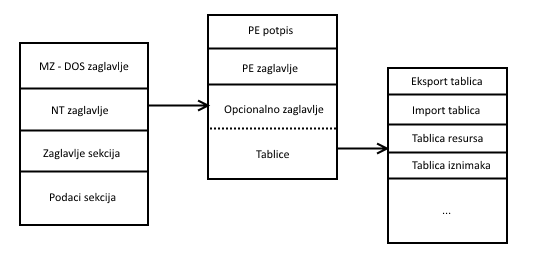
\includegraphics[width=10cm, height=6cm]{slike/pe_format}
\caption{PE format}
\label{fig:pe_format} 
\end{figure} 

\pagebreak										% U LaTeX-u se rijetko ubacuju prijelomi stranica!

Znači, kao što je vidljivo na slici \ref{fig:pe_format}, svaka PE
datoteka može se podijeliti na sljedeće dijelove:

\begin{itemize}
\item MZ-DOS zaglavlje
\item NT zaglavlje
	\begin{itemize}
	\item PE zaglavlje
	\item Opcionalno zaglavlje
	\item Tablice
	\end{itemize}
\item Zaglavlje sekcija									% Doista idu prvo sva zaglavlja, pa svi podaci? Ili su zaglavlje+podaci u paketu?
\item Podaci sekcija
\end{itemize}

\pagebreak

\subsection{Relokacije i Relativne Virtualne Adrese}

Prije samog opsa PE formata datoteka potrebno je ukratko
opisati pojmove relokacija i relativnih virtualnih adresa.
Navedeni pojmovi su od ključne važnosti za učitavanje PE datoteka
u memoriju te ih je potrebno razumjeti kako bi se ideja o
implementaciji permutacija nad izvršnim kodom PE datoteka mogla
ostvariti. U nastavku su dane najvažnije informacije o oba pojma.			% Rekao bi da su objašnjeni, a ne da su dane informacije

\subsubsection{Relativne Virtualne Adrese}
\label{sct:rva}

Unutar PE datoteka postoje mnoga mjesta u izvršnom kodu gdje je
potrebno definirati memorijske adrese. Uzmimo za primjer neku
globalnu varijablu. Kako bi se ta ista varijabla mogla
referencirati potrebno je znati njezinu adresu u memoriji. Iako
za sve PE datoteke postoji preferirana adresa na koju se datoteka
učitava u memoriju, svaka PE datoteka se može učitati na bilo
koju adresu unutar adresnog prostora procesa. Iz tog razloga jako
je loše koristiti apsolutne adrese te mora postojati način preko
kojega je moguće specificirati adrese koje su neovisne o lokaciji
na koju je datoteka učitana u memoriju.

Iz prethodno navedenih razloga, uvedene su relativne virtualne
adrese. Pojednostavljeno, relativne virtualne adrese su pomaci u
odnosu na početnu adresu na koju je PE datoteka učitana u
memoriju. Za primjer, uzmimo sljedeću situaciju: Neka je PE
datoteka učitana na adresu \emph{0x400000} u memoriji te neka je
njena sekcija (\ref{sec:sekcije}) s izvršnim kodom učitana na				% Razmaci prije i poslije zagrada!
adresi \emph{0x401000}. Relativna virtualna adresa sekcije se iz
navedenih podataka računa na sljedeći način: (Adresa					% Prepisati, nije potrebno ovako raspisivati!
sekcije)\emph{0x401000} - (Adresa datoteke)\emph{0x400000} =
(Relativna virtualna adresa)\emph{0x1000}.

Obrnuti proces, tj. pretvorbu relativne virtualne adrese u
apsolutnu adresu provodi se tako što se relativna virtualna
adresa (\emph{0x1000}) zbroji sa adresom na koju je datoteka
učitana u memoriju (\emph{0x400000}). Ta apsolutna adresa naziva			% Ta adresa, bez virtualna?
se virtualnom adresom. Na odsječku koda \ref{lst:primjer_rva}				% Sve ``odsječke koda'' zamijeniti s ``ispis''
prikazan je primjer relativne virtualne adrese. Niz okteta
\emph{E8 45010000} označava operacijski kod \emph{CALL}
instrukcije. Navedena instrukcija poziva funkciju koja se nalazi
na pomaku \emph{0x00000145} od trenutne pozicije. Taj pomak
naziva se relativna adresa s obzirom na trenutnu poziciju
(\emph{CALL} instrukcija). 

\begin{lstlisting}[frame=single, caption=Primjer relativne virtualne adrese, label={lst:primjer_rva}]
6A 00	                      PUSH 0
E8 45010000                   CALL <JMP.&KERNEL32.GetModuleHandleA>
A3 54304000                   MOV DWORD PTR DS:[403054],EAX
\end{lstlisting}

\subsubsection{Relokacije}

Sada kada je objašnjen pojam relativnih virtualnih adresa, moguće
je opisati pojam relokacija. Kao što je već navedeno, svaka PE
datoteka sadrži značajan broj memorijskih adresa preko kojih
referenciraju varijable, funkcije itd. Kod DLL-ova, velik broj				% Doista? DLL-ovi koriste apsolutne adrese?
adresa je apsolutan te je izračunat s obzirom na preferiranu
adresu na koju se datoteka pokušava učitati u memoriju. Te adrese
će biti ispravna samo u slučaju kada se PE datoteka uistinu učita
na preferiranu adresu.

Međutim, ukoliko se PE datoteka učita na neku drugu memorijsku
adresu unutar adresnog prostora, tada sve apsolutne adrese više
neće biti ispravne te je potrebno provesti dodatne korake kako bi
program radio ispravno. 

Upravo tu do izražaja dolaze osnovne relokacije. Cilj osnovnih
relokacija je obavijestiti program za učitavanje
(engl. \emph{loader}) o svim lokacijama unutar datoteke koje je
potrebno modificirati ukoliko se datoteka ne učita na preferiranu
adresu. To je ostvareno na način što program za učitavanje zna da
postoji lista unutar PE datoteke koja sadrži informacije o tim
lokacijama.

Kako bi bilo jasnije, proučimo sljedeći primjer: Neka u izvršnom
kodu postoji sljedeća instrukcija koja učitava vrijednost sa neke
memorijske lokacije u ECX registar (odsječak koda
\ref{lst:base_reloc})

\begin{lstlisting}[frame=single, caption=Primjer za relokacije, label={lst:base_reloc}]
00401020: 8B 0D 34 D4 40 00  mov ecx,dword ptr [0x0040D434]
\end{lstlisting}

Kao što je vidljivo instrukcija se nalazi na adresi
\emph{0x00401020} te je duga šest okteta. Prva dva okteta
(\emph{0x8D 0x0D}) sačinjavaju operacijski kod instrukcije dok				% Krivi oktet!
ostala četiri okteta čine apsolutnu adresu (\emph{0x0040D434}). U
ovom slučaju PE datoteka je učitana na preferiranu adresu koja
iznosi \emph{0x00400000} te se varijabla koju je potrebno učitati
nalazi na relativnoj virtualnoj adresi iznosa \emph{0xD434}.

Ukoliko se spomenuta PE datoteka uistinu učita na
\emph{0x00400000}, navedena instrukcija će raditi bez problema.
Međutim, recimo da se datoteka učita na adresu \emph{0x00500000}.
U tom slučaju je šest okteta koji čine adresu potrebno
promijeniti tako da pokazuju na adresu \emph{0x0050D434}.

Način na koji se provodi promjena adrese je sljedeći: Program za
učitavanje uspoređuje preferiranu adresu na koju je datoteku
potrebno učitati te stvarnu adresu na koju je ista učitana. Na
taj način izračuna se razlika koja u ovom slučaju iznosi
\emph{0x00100000}. Tu razliku moguće je zatim dodati adresi
\emph{0x0040D434} kako bi se dobila stvarna adresa na kojoj je
vrijednost varijable pohranjena. Ukratko, u tablici relokacija
(tablica \ref{tbl:imgDataDir}) postoji informacija o potrebnoj
relokaciji za adresu \emph{0x00401022}.

Ovime je objašnjeno kako funkcioniraju relokacije za PE datoteke.
Valja još napomenuti način na koji su informacije o relokacijama
pohranjene u samoj PE datoteci. Svaka relokacija može se opisati
jednostavnom strukturom \emph{IMAGE\_BASE\_RELCOATION} čiji
sadržaj je moguće vidjeti u odsječku koda \ref{lst:imgBaseReloc}.

\begin{lstlisting}[frame=single, caption=IMAGE\_BASE\_RELOCATION struktura, label={lst:imgBaseReloc}]
typedef struct _IMAGE_BASE_RELOCATION {
    DWORD   VirtualAddress;
    DWORD   SizeOfBlock;
} IMAGE_BASE_RELOCATION;
typedef IMAGE_BASE_RELOCATION;
\end{lstlisting}

Svaka \emph{IMAGE\_BASE\_RELOCATION} struktura sastoji se od dva			% Ovo mi nije jasno!?
elementa. Prvi element, \emph{VirtualAddress}, sadrži relativnu
virtualnu adresu koja označava početak bloka memorije na koji
treba primijeniti relokacije. Element \emph{SizeOfBlock} označava
koliko okteta zauzimaju relokacijske informacije za taj konkretni
blok. 

Nakon svake \emph{IMAGE\_BASE\_RELOCATION} strukture nalazi se
varijabilan broj 16-bitnih vrijednosti. Svaka od 16-bitnih
vrijednosti može se rastaviti na dva dijela:

\begin{itemize}
\item Gornja 4 bita označavaju tip relokacije koji treba
primijeniti. Postoji nekoliko tipova relokacija te su svi opisani
u službenoj specifikaciji za PE format \citep{pe_spec}.

\item Donjih 12 bitova označavaju pomak u odnosu na element
\emph{VirtualAddress}, iz strukture
\emph{IMAGE\_BASE\_RELCOATION}, na koji je potrebno primijeniti
relokaciju.
\end{itemize}

Ovime su dane najosnovnije informacije vezane za relativne
virtualne adrese i relokacije. U nastavku ovog poglavlja opisana
su osnovna zaglavlja i elementi PE datoteka.

\pagebreak

\subsection{MZ-DOS Zaglavlje}

MZ-DOS zaglavlje je prvo zaglavlje kod PE datoteka te se sastoji
od dva dijela. Prvi dio opisan je strukturom
\emph{IMAGE\_DOS\_HEADER} čiji sadržaj je prikazan na odsječku
koda \ref{lst:imgDosHeader}.

\begin{lstlisting}[frame=single, caption=IMAGE\_DOS\_HEADER struktura, label={lst:imgDosHeader}]
typedef struct _IMAGE_DOS_HEADER {      // DOS .EXE header
	WORD   e_magic;                     // Magic number
	WORD   e_cblp;                      // Bytes on last page of file
	WORD   e_cp;                        // Pages in file
	WORD   e_crlc;                      // Relocations
	WORD   e_cparhdr;                   // Size of header in paragraphs
	WORD   e_minalloc;                  // Minimum extra paragraphs needed
	WORD   e_maxalloc;                  // Maximum extra paragraphs needed
	WORD   e_ss;                        // Initial (relative) SS value
	WORD   e_sp;                        // Initial SP value
	WORD   e_csum;                      // Checksum
	WORD   e_ip;                        // Initial IP value
	WORD   e_cs;                        // Initial (relative) CS value
	WORD   e_lfarlc;                    // File address of relocation table
	WORD   e_ovno;                      // Overlay number
	WORD   e_res[4];                    // Reserved words
	WORD   e_oemid;                     // OEM identifier (for e_oeminfo)
	WORD   e_oeminfo;                   // OEM information; e_oemid specific
	WORD   e_res2[10];                  // Reserved words
	LONG   e_lfanew;                    // File address of new exe header
} IMAGE_DOS_HEADER, *PIMAGE_DOS_HEADER;
\end{lstlisting}

Iako struktura \emph{IMAGE\_DOS\_HEADER} sadrži 31 element, valja
napomenuti kako su, za potrebe ovog rada, od osobite važnosti
samo elementi na prvom i posljednjem mjestu u strukturi. Element
na prvom mjestu u strukturi (\emph{e\_magic}) označava potpis PE
datoteka te uvijek mora sadržavati vrijednost "MZ", tj. 0x5A4D u
heksadecimalnom obliku. Ukoliko su ta prva dva okteta različita
od "MZ", PE datoteka se ne smatra valjanom. Posljednji element u
strukturi (\emph{e\_lfanew}) je najvažniji element
\emph{IMAGE\_DOS\_HEADER} strukture jer pokazuje na početak				% Kako se računa taj početak?
sljedećeg zaglavlja, tj. na \emph{NT zaglavlje}.

Osim \emph{IMAGE\_DOS\_HEADER} strukture, MZ-DOS zaglavlje sadrži
i tzv. DOS dopunski program (engl.\emph{DOS stub
program})\citep{dos_stub}. DOS dopunski program ima samo jednu
namjenu, a to je da ispiše kratak tekst i završi sa izvršavanjem
ukoliko se PE datoteka pokuša pokrenuti na 16-bitnom DOS računalu.
Potreba za time seže još u same početke razvoja Windows
operacijskog sustava kakav se koristi danas. Razvoj PE datoteka
započeo je još dok su računala sa DOS-om bila prilično raširena u
upotrebi, te kako se ne bi utjecalo na strukturu PE formata,
uveden je DOS dopunski program koji upozorava korisnika o
pokušaju izvršavanja PE datoteke na DOS stroju. DOS dopunski
program najčešće je veličine 128 okteta i sadrži tekst "This
program cannot be run in DOS mode". Primjer izgleda DOS dopunskog
programa moguće je vidjeti na slici \ref{fig:dos_stub}.

\begin{figure}[!ht]
\centering
\setlength\fboxsep{0pt}
\setlength\fboxrule{0.5pt}
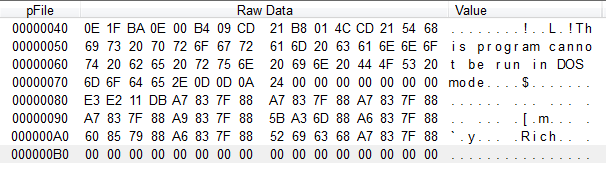
\includegraphics[width=10cm, height=4cm]{slike/dos_stub}
\caption{DOS dopunski program}
\label{fig:dos_stub} 
\end{figure}

\subsection{NT Zaglavlje}

Sljedeće zaglavlje u PE datotekama, \emph{NT zaglavlje}, sadrži
najvažnije informacije vezane uz datoteku. Kao što prikazuje
slika \ref{fig:pe_format}, \emph{NT zaglavlje} se sastoji od 3
ključna dijela:

\begin{itemize}
\item Potpis PE zaglavlja
\item PE zaglavlje
\item Opcionalno zaglavlje
\end{itemize} 

Potpis PE zaglavlja, slično kao i kod MZ-DOS zaglavlja,
sačinjavaju 4 okteta (0x00004550) koji predstavljaju znakovni niz
"PE". Kako bi PE datoteka bila valjana, nužno je da potpis
sadrži valjanu vrijednost. 

PE zaglavlje (engl.\emph{PE File Header}) definirano je unutar
strukture \emph{IMAGE\_FILE\_HEADER}. Veličina zaglavlja je 20
	okteta te je njegovu strukturu moguće vidjeti na odsječku koda				% Te je njegova struktura prikazana na ispisu
\ref{lst:imgFileHeader}

\begin{lstlisting}[frame=single, caption=IMAGE\_FILE\_HEADER struktura, label={lst:imgFileHeader}]
typedef struct _IMAGE_FILE_HEADER {
	WORD    Machine;
	WORD    NumberOfSections;
	DWORD   TimeDateStamp;
	DWORD   PointerToSymbolTable;
	DWORD   NumberOfSymbols;
	WORD    SizeOfOptionalHeader;
	WORD    Characteristics;
} IMAGE_FILE_HEADER, *PIMAGE_FILE_HEADER;
\end{lstlisting}

U tablici \ref{tbl:imgFileHdr} nalazi se opis pojedinih elemenata
\emph{IMAGE\_FILE\_HEADER} strukture.

\pagebreak

\begin{table}[htb]
\small
\caption{IMAGE\_FILE\_HEADER struktura - opis elemenata}
\label{tbl:imgFileHdr}
\centering
\begin{tabular}{|l|l|l|p{6cm}|}
\hline
Pomak & Veličina & Element & Opis \\ \hline
0 & 2 & Machine & Broj koji definira stroj(arhitekturu) za koju je datoteka namijenjena \\ \hline
2 & 2 & NumberOfSections & Označava koliko sekcija postoji u datoteci. Nakon NT zaglavlja slijedi toliki broj zaglavlja sekcija. \\ \hline
4 & 4 & TimeDateStamp & Vrijeme i datum kada je datoteka kreirana \\ \hline
8 & 4 & PointerToSymbolTable & Posmak do tablice simbola karakteristične za COFF format. Sadrži 0 ukoliko tablica ne postoji. \\ \hline
12 & 4 & NumberOfSymbols & Broj elemenata u tablici simbola. \\ \hline
16 & 2 & SizeOfOptionalHeader & Označava veličinu opcionalnog zaglavlja. Opcionalno zaglavlje slijedi odmah nakon PE zaglavlja. \\ \hline
\end{tabular}
\end{table}

Nakon PE zaglavlja dolazi opcionalno zaglavlje. Opcionalno
zaglavlje sadrži veliki broj elemenata od kojih nisu svi nužni za
razumijevanje ovog rada. Zbog toga su u ovom odjeljku opisani
samo najvažniji od njih. Opcionalno zaglavlje definirano je
unutar strukture \emph{IMAGE\_OPTIONAL\_HEADER}. Izgled navedene
strukture prikazan je na odsječku koda \ref{lst:imgOptHeader}.

%% Svuda promijeniti da pise "Strukutra XYZ"

\begin{lstlisting}[frame=single, caption=IMAGE\_OPTIONAL\_HEADER struktura, label={lst:imgOptHeader}]
typedef struct _IMAGE_OPTIONAL_HEADER {
	WORD    Magic;
	BYTE    MajorLinkerVersion;
	BYTE    MinorLinkerVersion;
	DWORD   SizeOfCode;
	DWORD   SizeOfInitializedData;
	DWORD   SizeOfUninitializedData;
	DWORD   AddressOfEntryPoint;
	DWORD   BaseOfCode;
	DWORD   BaseOfData;
	DWORD   ImageBase;
	DWORD   SectionAlignment;
	DWORD   FileAlignment;
	WORD    MajorOperatingSystemVersion;
	WORD    MinorOperatingSystemVersion;
	WORD    MajorImageVersion;
	WORD    MinorImageVersion;
	WORD    MajorSubsystemVersion;
	WORD    MinorSubsystemVersion;
	DWORD   Win32VersionValue;
	DWORD   SizeOfImage;
	DWORD   SizeOfHeaders;
	DWORD   CheckSum;
	WORD    Subsystem;
	WORD    DllCharacteristics;
	DWORD   SizeOfStackReserve;
	DWORD   SizeOfStackCommit;
	DWORD   SizeOfHeapReserve;
	DWORD   SizeOfHeapCommit;
	DWORD   LoaderFlags;
	DWORD   NumberOfRvaAndSizes;
	IMAGE_DATA_DIRECTORY DataDirectory[IMAGE_NUMBEROF_DIRECTORY_ENTRIES];
} IMAGE_OPTIONAL_HEADER32, *PIMAGE_OPTIONAL_HEADER32;
\end{lstlisting}

Najvažniji dijelovi opcionalnog zaglavlja i njihovi opisi			% Izbjegavati to "navedeni su u nastavku", samo kazes da "su", i to je to...
navedeni su u nastavku:

\begin{itemize}
\item \emph{SizeOfCode}: Veličina \emph{code} sekcije. Ukoliko
postoji više sekcija koje sadrže izvršni kod, tada ova vrijednost
sadržava sve zbrojene veličine.

\item \emph{AddressOfEntryPoint}: Označava adresu unutar sekcije
sa izvršnim kodom od koje kreće izvršavanje programa. Valja
napomenuti kako ovo polje ne sadrži stvarnu adresu već tzv.
relativnu virtualnu adresu. Kao što je spomenuto u \ref{sct:rva}
relativna virtualna adresa označava pomak od bazične adrese na
koju je datoteka učitana u memoriju.

\item \emph{BaseOfCode}: Sadrži relativnu virtualnu adresu od
početka sekcije sa izvršnim kodom. Navedena adresa vrijedi tek od
trenutka kada je datoteka učitana u memoriju.

\item \emph{ImageBase}: Preferirana adresa prvog bajta datoteke
prilikom učitavanja u memoriju. Navedena vrijednost mora biti
višekratnik 64K. Zadana vrijednost za DLL-ove iznosi 0x10000000,
dok za izvršne datoteke iznosi 0x00400000.

\item \emph{SectionAlignment}: Poravnanje sekcija jednom kada je
datoteka učitana u memoriju. Ova vrijednost mora biti veća ili
jednaka vrijednosti \emph{FileAlignment}.

\item \emph{FileAlignment}: Poravnanje sekcija dok se datoteka
nalazi na disku, znači dok nije učitana u memoriju. Zadana
vrijednost za ovaj element je 512, iako može varirati između 2 i
64K.

\item \emph{SizeOfImage}: Označava ukupnu veličinu, u oktetima,
datoteke jednom kada je učitana u memoriju. Mora biti višekratnik
elementa \emph{SectionAlignment}.

\item \emph{SizeOfHeader}: Označava ukupnu veličinu PE zaglavlja,
MZ-DOS dopunskog programa te zaglavlja sekcija. Mora biti
višekratnik elementa \emph{FileAlignment}.

\item \emph{NumberOfRvaAndSizes}: Element koji označava koliko
podatkovnih tablica slijedi nakon opcionalnog zaglavlja.
\end{itemize}

Kao što je već spomenuto, na kraju opcionalnog zaglavlja dolazi popis podatkovnih tablica u PE datoteci. Maksimalan broj tablica iznosi 16. Svaka tablica opisana je preko \emph{IMAGE\_DATA\_DIRECTORY} strukture čiji opis se može vidjeti na odsječku koda \ref{lst:dataDir}

\begin{lstlisting}[frame=single, caption=IMAGE\_DATA\_DIRECTORY struktura, label={lst:dataDir}]
typedef struct _IMAGE_DATA_DIRECTORY {
	DWORD   VirtualAddress;
	DWORD   Size;
} IMAGE_DATA_DIRECTORY, *PIMAGE_DATA_DIRECTORY;
\end{lstlisting}

Svaka \emph{IMAGE\_DATA\_DIRECTORY} struktura sastoji se od dva
elementa. Prvi element, \emph{VirtualAddress}, označava relativnu
virtualnu adresu do tablice u memoriji. Znači, radi se o pomaku
od početne adrese na koju je PE datoteka učitana u memoriju.
Drugo polje, \emph{Size}, označava veličinu tablice u oktetima.

Važna stvar za napomenuti je kako broj tablica nije fiksan.
Ukoliko postoji potreba za pretraživanjem direktorija tablica,
potrebno je provjeriti vrijednost \emph{NumberOfRvaAndSizes} u
opcionalnom zaglavlju prije nego se krene u potragu za određenom
tablicom. Naziv i kratak opis svih podatkovnih tablica prikazan
je na tablici \ref{tbl:imgDataDir}.

{\small
\begin{longtable}{|l|p{6cm}|}
\caption{Popis tablica u opcionalnom zaglavlju} \label{tbl:imgDataDir} \\
\hline
Tablica & Opis \\ \hline
Eksport Tablica & Adresa i veličina tablice koja opisuje eksport funkcije i DLL-ove. \\ \hline
Import Tablica &  Adresa i veličina tablice koja opisuje import funkcije i DLL-ove. \\ \hline
Tablica Resursa & Adresa i veličina tablice koja sadrži informacije o resursima. \\ \hline
Tablica Iznimaka & Sadrži adresu i veličinu tablice zadužene za iznimke. Tablica pokazuje na adrese funkcija koje su zadužene za rukovanje iznimkama. \\ \hline
Tablica Certifikata & Adresa i veličina tablice zadužene za certifikate. Ne mapira se u memoriju. \\ \hline
Relokacijska Tablica & Sadrži adresu i veličinu tablice u kojoj su sačuvani podaci o relokacijama. \\ \hline
Debug Tablica & Sadrži podatke o tablici koja sadrži informacije o otklanjanju grešaka. Ne mapira se u memoriju. \\ \hline
Arhitektura & Adresa i veličina tablice koja sadrži podatke o arhitekturi sustava. \\ \hline
Global Ptr & Sadrži relativnu virtualnu adresu vrijednosti koju je potrebno spremiti u registar globalnog pokazivača (engl.\emph{Global Pointer Register}) na procesoru. Polje veličine u ovom slučaju mora biti postavljeno na 0. \\ \hline
TLS Tablica & Sadrži adresu i veličinu TLS tablice (engl.\emph{Thread Local Storage}) \\ \hline
Tablica s konfiguracijom & Sadrži adresu i veličinu tablice koja pohranjuje informacije o postavkama na koje treba obratiti pažnju prilikom učitavanja datoteke u memoriju. \\ \hline
Tablica spremnih importa(engl.\emph{Bound Import}) & Radi se o opcionalnoj tablici koja sadrži informacije o import funkcijama i DLL-ovima koji su unaprijed učitani u memoriju na dobro poznate adrese te ih radi toga nije potrebno ponovno učitavati već se mogu odmah koristiti. \\ \hline
IAT tablica & Radi se o dijelu Import tablice. Konkretno, IAT (engl.\emph{Import Address Table}) sadrži popis adresa na kojima se nalaze funkcije učitane iz raznih DLL-ova koje program koristi. \\ \hline
Tablica odgođenih importa & Sadrži informacije o importima koji se naknadno mogu učitati u memoriju. Djeluje kao dodatak import tablice. \\ \hline
CLI Tablica & Sadrži adresu i veličinu tablice koja se uglavnom koristi kod .NET aplikacija. \\ \hline
Rezervirano & Rezervirano za potrebe operacijskog sustava. \\
\hline
\end{longtable}
}
\pagebreak

\subsection{Sekcije}
\label{sec:sekcije}

Zaglavlje sekcija i njihovi podaci zauzimaju najviše prostora
kako unutar PE datoteke na disku, tako i unutar memorije jednom
kada se datoteka učita. Lista zaglavlja sekcija slijedi odmah
nakon opcionalnog zaglavlja. Takav raspored je nužan, jer niti
jedno polje u PE zaglavlju ne sadrži informaciju o točnom odmaku
tablice sekcija. Zbog toga se koristi element
\emph{SizeOfOptionalHeader} kako bi se pronašao točan pomak do
zaglavlja sekcija. Svaka sekcija opisana je pomoću
\emph{IMAGE\_SECTION\_HEADER} strukture. Sadržaj navedene
strukture prikazan je u odsječku koda \ref{lst:imgSectionHeader}.

\begin{lstlisting}[frame=single, caption=IMAGE\_SECTION\_HEADER struktura, label={lst:imgSectionHeader}]
typedef struct _IMAGE_SECTION_HEADER {
	BYTE    Name[IMAGE_SIZEOF_SHORT_NAME];
	union {
		DWORD   PhysicalAddress;
		DWORD   VirtualSize;
	} Misc;
	DWORD   VirtualAddress;
	DWORD   SizeOfRawData;
	DWORD   PointerToRawData;
	DWORD   PointerToRelocations;
	DWORD   PointerToLinenumbers;
	WORD    NumberOfRelocations;
	WORD    NumberOfLinenumbers;
	DWORD   Characteristics;
} IMAGE_SECTION_HEADER, *PIMAGE_SECTION_HEADER;
\end{lstlisting}

Prikazana \emph{IMAGE\_SECTION\_HEADER} struktura sastoji se od
10 elemenata. U nastavku slijedi opis svakog od navedenih				% Značenja pojedinih polja su sljedeća:
elemenata:

\begin{itemize}

\item \emph{Name}: Označava ime sekcije. Imena sekcija najčešće
započinju sa točkom te su oblika ".text", ".code", ".rsrc",
".data" itd. Iako ime sekcije u početku dosta pomaže prilikom
shvaćanja koji tipovi podataka i informacija se nalaze unutar
pojedine sekcije, ono ne mora nužno postojati ili može biti
proizvoljno. Mnogo puta je određene PE datoteke, koje su pakirane
ili zaštičene na neki način, moguće identificirati samo po
neuobičajenim imenima sekcija. Valja još napomenuti kako je
duljina imena sekcije ograničena na 8 okteta (znakova).

\item \emph{VirtualSize}: Navedeno polje označava ukupnu veličinu
sekcije koju ista zauzima u memoriji kada je PE datoteka učitana.
Ukoliko je ovo polje veće od polja \emph{SizeOfRawData}, tada se
na višak prostora u memoriji postavljaju nule.

\item \emph{VirtualAddress}: Relativna virtualna adresa koja
označava pomak do prvog okteta sekcije jednom kada je ista
učitana u memoriju.

\item \emph{SizeOfRawData}: Veličina, u oktetima, sekcije na
disku. Za izvršne datoteke, ova vrijednost mora biti višekratnik
elementa \emph{FileAlignment} iz opcionalnog zaglavlja. Ukoliko
je ova vrijednost manja od elementa \emph{VirtualSize}, tada se
ostatak sekcije nadopuni nulama prilikom učitavanja u memoriju.
Ako sekcija koristi ne inicijalizirane podatke, tada ovaj
parametar treba biti nula.

\item \emph{PointerToRawData}: Pokazivač na prvi oktet sekcije
dok se ista nalazi na disku. Za izvršne datoteke, ova vrijednost
mora piti višekratnik parametra \emph{FileAlignment} iz
opcionalnog zaglavlja. Ako sekcija koristi ne inicijalizirane
podatke, tada ovaj parametar treba biti nula.

\item \emph{PointerToRelocations}: Pokazivač na relokacije za
dotičnu sekciju. Ukoliko se radi o izvršnoj datoteci a ne o DLL-u
te ukoliko relokacije ne postoje, ovaj parametar se postavlja na
nulu.

\item \emph{PointerToLineNumbers}: Pokazivač na skup podataka
koji stvaraju vezu između određenih virtualnih adresa i linija u
datoteci s izvornim kodom na koje se te adrese odnose.

\item \emph{NumberOfRelocations}: Sadrži broj relokacijskih unosa
za promatranu sekciju.

\item \emph{NumberOfLineNumbers}: Sadrži broj veza između
virtualnih adresa u sekciji i linija u datoteci s izvornim kodom.

\item \emph{Characteristics}: Polje zastavica koje označava neke
karakteristike sekcije. Neke od mogućih karakteristika su:

\begin{itemize}
\item IMAGE\_SCN\_CNT\_CODE: Oznaka da sekcija
sadrži izvršni kod.

\item IMAGE\_SCN\_CNT\_INITIALIZED\_DATA:
Oznaka da sekcija sadrži inicijalizirane podatke.

\item IMAGE\_SCN\_CNT\_UNINITIALIZED\_DATA: Oznaka da sekcija sadrži
neinicijalizirane podatke.

\item IMAGE\_SCN\_MEM\_EXECUTE: Oznaka za dozvolu da se sadržaj
sekcije tretira kao izvršni kod, te se time može i izvršavati.

\item IMAGE\_SCN\_MEM\_READ: Oznaka kako se sadržaj sekcije samo
može čitati, a ne mijenjati i izvršavati.

\item IMAGE\_SCN\_MEM\_WRITE: Oznaka kako se sadržaj
sekcije može mijenjati, ali ne i izvršavati.
\end{itemize}

\end{itemize}



\section{Alati}									% Ovdje se počinje o svim alatima, pa razvoj, pa opet svi alati... to malo bolje strukturirati...

Postoji velik broj alata za rad sa PE datotekama. Ukoliko se želi
započeti sa razvojem vlastitih alata za rad sa PE datotekama,
Microsoft nudi značajan broj već postojećih makroa, funkcija i
struktura specijaliziranih za rad sa PE formatom. Navedeno se
nalazi unutar zaglavlja \emph{WINNT.H} i \emph{Windows.h}.

Osim razvoja vlastitih alata, postoji i značajan broj već
postojećih alata koji olakšavaju analizu pojedinih dijelova PE
datoteka. Neki od njih su:

\begin{itemize}
\item PeView: Alat koji pregledno prikazuje strukturu bilo koje			% U literaturu staviti linkove na alate i pozvati se na reference!
PE datoteke. Ne nudi mogućnost promjene pojedinih elemenata u PE
datoteci, ali značajno olakšava snalaženje unutar pojedinih
dijelova datoteke.

\item LordPE: Moćan alat koji osim analize pojedinih elemenata u		% Umjesto "moćan" staviti "s mnoštvom mogućnosti" ili nešto slično
PE datoteci, nudi i mogućnost promjene vrijednosti čime se dobiva
potpuno nova PE datoteka sa novim svojstvima.

\end{itemize}

\chapter{Postojeći Mehanizmi Zaštite}

Cilj ovog poglavlja je dati kratak uvod u postojeće mehanizme
zaštite koji značajno pomažu u sprječavanju napada usmjerenih na		% Ovo je malo krivo rečeno "na memoriju", na propuste u radu s memorijom ili nešto slično
memoriju. Konkretno, radi se o mehanizmima: ASLR (engl.
\emph{Address Space Layout Randomization}), DEP (engl. \emph{Data
Execution Prevention}) i ASLP (engl.\emph{Address Space Layout
Permutation}), pri čemu je ASLP usmjeren striktno na Linux
operacijski sustav, ali zbog sličnosti sa alatom koji ovdje
razvijamo smatram da je potrebno reći nešto i o tome. 

\section{ASLR}
\label{sct:aslr}

ASLR je sigurnosni mehanizam čiji cilj je zaštita sustava od
napada usmjerenih na memoriju poput preljev spremnika (engl.
\emph{Buffer Overflow Attack}) i programiranja temeljenog na
"ret" blokovima. Način na koji ASLR štiti od napada je taj što se
ključni dijelovi programa učitavaju na slučajne lokacije u
memoriji. Ti ključni dijelovi su početna adresa na koju je
izvršna datoteka učitana, pozicija vanjskih biblioteka, pozicija
gomile (engl. \emph{Heap}) te pozicija stoga (engl.\emph{Stack})		% Na niz mjesta nema razmaka iza točke...
unutar procesnog adresnog prostora.

ASLR značajno otežava napadačima pronalaženje točnih adresa na
kojima se nalazi ranjivi programski kod. Za primjer, napadači
koji pokušavaju izvesti napad temeljen na "ret" blokovima
(engl.\emph{Return Oriented Programming})\citep{rop_official}
moraju pronaći točne memorijske lokacije pojedinih blokova kako
bi ih bili u mogućnosti izvesti. Također, napadači koji
pokušavaju izvršiti kod koji su uspjeli ubaciti na stog moraju
prvo znati gdje se unutar adresnog prostora stog nalazi. ASLR
onemogućava pronalaženje točnih adresa te su napadači u situaciji
gdje moraju pogađati točne adrese, pri čemu loš pogodak uzrokuje
pogrešku u aplikaciji te njezino gašenje.

Sigurnost koju nudi ASLR počiva na malenoj vjerojatnosti da će
napadač uspjeti pogoditi nasumično raspoređene dijelove programa.
Sigurnost je u ASLR-u moguće povećati na dva načina: povećanje
prostora u virtualnoj memoriji unutar kojega se vrši nasumičan
raspored programskih dijelova, te smanjenje perioda unutar kojega
je potrebno ponoviti novi nasumični raspored. 

ASLR se unutar Windows Vista i 7 provodi na 3 razine: učitavanje
izvršne datoteke ili DLL-a na nasumičnu adresu, učitavanje gomile
na nasumičnu adresu te učitavanje stoga na nasumična adresu. 

Proces odabira nasumične početne adrese provodi se na sljedeći
način: Prilikom učitavanja PE(engl. \emph{Portable Executable})			% Razmak prije zagrade!
datoteke u memoriju, Windows operacijski sustav pročita
vrijednost TSC(engl. \emph{Time Stamp Counter}) registra
procesora. TSC registar sadrži broj ciklusa procesora nakon
zadnjeg pokretanja. Taj broj se zatim pomiče za četiri mjesta te
se provodi operacija \emph{mod 254} i dodaje 1. Dobivena
vrijednost se zatim množi sa \emph{64KB = 65536} te se dobiveni
rezultat koristi kao početna adresa za program. Na taj način,
postoji 256 različitih lokacija na koje je moguće učitati izvršnu
datoteku. Kod DLL-ova(engl. \emph{Dynamic Link Library}) je
postupak malo drugačiji. Naime, pošto se DLL-ovi dijele u
memoriji između više procesa, potrebno je imati drugačiji način
izračuna početne adrese. Za potrebe jednostavnijeg objašnjenja
uvodi se vrijednost \emph{var}. To je vrijednost koja se računa
samo jednom prilikom pokretanja sustava na način da se uzima
vrijednost TSC registra te se ona pomiče i maskira na vrijednost
veličine 8 bita. Pošto se svi DLL-ovi učitavaju u dijeljeni
memorijski prostor u rasponu od \emph{0x50000000 - 0x78000000},
formula po kojoj se računa adresa prvog učitanog DLL-a je
\emph{0x78000000 - var * 0x100000}. Redoslijed prema kojemu se
učitavaju DLL-ovi je također nasumičan jer se prije ASLR-a kao
prvi DLL učitavao \emph{ntdll.dll}. Problem kod toga je što bi
bilo jednostavno pronaći pomak do modula ako se zna početna
adresa od \emph{ntdll.dll}. 

Učitavanje stoga na nasumičnu adresu provodi se za svaku stvorenu
dretvu. Obavlja se na način da se unaprijed pronalaze 32
odgovarajuće lokacije u memoriji. U trenutku stvaranja stoga,
uzima se vrijednost TSC registra te se ona pomiče i maskira na
veličinu 5 bitova na osnovu kojih se odabire jedna od 32 moguće
lokacije. Nakon što je adresa odabrana, izvede se novih 9 bitova
iz vrijednosti pročitane iz TSC registra te se na osnovu njih
izračuna konačna adresa stoga u memoriji.

Na kraju se provodi učitavanje gomile na nasumičnu adresu. To se
provodi na način da se pročita vrijednost TSC registra te se iz
te vrijednosti izvede 5-bitna vrijednost koja se zatim množi sa
64KB, pri čemu se dobiva mogući raspon od \emph{0x00000000 -
0x001F0000} adresa. Na Slici \ref{fig:aslr} prikazan je raspored
DLL-ova u adresnom prostoru procesa između dva pokretanja
sustava.

\begin{figure}[!ht]
\centering
\setlength\fboxsep{0pt}
\setlength\fboxrule{0.5pt}
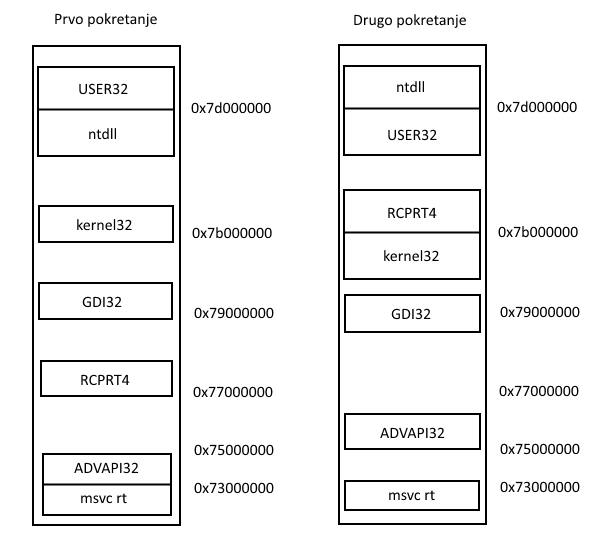
\includegraphics[width=10cm, height=10cm]{slike/aslr_v2}
\caption{Primjer ASLR-a između dva pokretanja}					% Primjer djelovanja ASLR-a između...
\label{fig:aslr} 
\end{figure} 

\section{DEP}
\label{sct:dep}

DEP(engl. \emph{Data Execution Prevention}) je skup programskih i
sklopovskih rješenja koji provodi dodatne provjere memorije radi
sprječavanja pokretanja zloćudnog koda u sustavu. Glavna prednost
DEP-a je sprječavanje pokretanja koda sa podatkovnih stranica.
DEP onemogućava pokretanje koda iz gomile ili sa stoga te se
pojavljuje u dva načina rada:

\begin{itemize}
\item Sklopovski pojačan DEP: prepoznaje pokretanje koda iz gomile ili sa stoga te generira iznimku kada do izvršavanja dođe.		% Detektira pokušaj izvršavanja (nečega) na stogu...
\item Programski pojačan DEP: može spriječiti da zloćudni kod koristi mehanizme za rukovanje iznimkama u sustavu Windows.
\end{itemize}

Hardverski pojačan DEP označava sve memorijske lokacije kao ne			% Maloprije je bio sklopovski... osim toga, jel "pojačan" ili "podržan"?
izvršne, osim ako neka od njih eksplicitno ne sadrži programski			% neizvršive...
kod. Ovaj oblik DEP-a oslanja se na procesor kako bi označio			% Procesor detektira pokušaj, a OS je taj koji označava...
memoriju atributom koji govori kako se iz nje ne bi smio
izvršavati programski kod.

Arhitektura procesora određuje način na koji je DEP implementiran
u sklopovlju i na koji označava stranicu u virtualnoj memoriji.			% te kako se označavaju neizvršive stranice...
Na taj način procesori koji podržavaju DEP mogu generirati
iznimku kada se počne izvršavati kod sa stranica označenih
odgovarajućim skupom atributa.

Kako bi spriječio izvršavanje, operacijski sustav Windows koristi
jedno od sljedećeg:

\begin{itemize}
\item Procesorska značajka zabrane izvršavanja(NX) - definirano od strane AMD-a
\item Bit za onemogućavanje izvršavanja(XD) - definirano od strane Intel-a
\end{itemize}

Kako bi procesor mogao koristiti navedene značajke, on mora
raditi u PAE(engl. \emph{Physical Address
Extension})\citep{pae_ms} načinu rada. Spomenuti način rada
omogućava 32-bitnom procesoru da adresira više od 4 giga-bajta
memorije. To se ostvaruje tako što se procesorska arhitektura
proširuje na način da se umjesto 32 bita za adrese koristi 36
bita. Valja još napomenuti kako operacijski sustav Windows
automatski omogućava PAE radi podrške za DEP. Time nije potrebno		% Na taj način korisnike ne mora eksplicitno omogućiti PAE...
tražiti od korisnika da zasebno omoguće PAE prilikom pokretanja
sustava.

Programski pojačan DEP je skup sigurnosnih provjera koje su
osmišljene radi sprječavanja zloćudnog koda koji iskorištava
mehanizme rukovanja iznimkama (engl. \emph{Structured Exception
Handling}). Ovaj oblik DEP-a primjenjiv je samo na procese iz
korisničkog načina rada. Glavna karakteristika softverski
pojačanog DEP-a je što može štiti samo ograničene sistemske
binarne datoteke.

U konačnici, DEP može značajno pomoći u sprječavanju sigurnosnih
upada. Pri tome, posebno može pomoći u situacijama gdje zloćudni
program ubacuje dodatni kod u neki proces te zatim pokušava
izvršiti taj kod. Ako je u takvom sustavu DEP omogućen, inicira
se iznimkama prilikom pokretanja dodatnog koda.

\section{ASLP}
\label{sct:aslp}

ASLP\citep{aslp} (engl.\emph{Address Space Layout Permutation})			% Razmak prije citata
je alat za operacijski sustav Linux koji omogućava pomicanje
(permutaciju) dijelova koda i podataka iz izvršnih ELF datoteka
na slučajno odabrane nove lokacije unutar izvršne ELF datoteke.
Time datoteka i dalje zadržava svoju funkcionalnost, ali je
njezin memorijski raspored promijenjen. Iz navedenoga se lako
može zaključiti kako je ASLP dosta sličan modulu za promjenu koda
koji se razvija u sklopu ovog rada s razlikom što je modul za
promjenu koda orijentiran na Microsoft Windows platformu. 

ASLP, također, kao ulaz prima izvršnu datoteku te provodi
permutacije nad svim sekcijama koje sadrže izvršni kod ili
podatke. ASLP provodi permutacije na dvije razine, tj. na razini
korisničkog prostora te na razini jezgre operacijskog sustava. U
nastavku ovog poglavlja detaljnije je opisan koncept iza obje
razine permutacije.

\subsection{Permutacija u Korisničkom Prostoru}

Temelj za permutaciju u korisničkom prostoru je program koji
mijenja lokaciju podatkovnih i izvršnih dijelova datoteke. Time
se u potpunosti mijenja memorijski raspored ELF datoteke, dok
njezina funkcionalnost ostaje ista.

Permutacija se u korisničkom prostoru provodi u dva koraka. U
prvom koraku se mijenjaju početne adrese podatkovnih i izvršnih
dijelova datoteke, dok se u drugom koraku provodi dodatna
permutacija unutar samih dijelova. U sklopu te dodatne
permutacije provodi se slučajna reorganizacija tijela funkcija
unutar dijela s izvršnim kodom, te reorganizacija statičnih i
globalnih varijabli unutar dijela s podacima. Glavni problem koji
se ovdje javlja (isto je i s modulom za promjenu koda koji			% Izbjegavati zagrade
razvijamo) je ažuriranje svih referenci među raznim objektima u
programu.

Program za permutaciju u korisničkom prostoru, osim same datoteke
nad kojom se permutacija provodi, prima i vrijednosti između 1 i
700K. Navedene vrijednosti bira korisnik i one se koriste
prilikom izračuna pomaka na koji treba postaviti podatkovne i
izvršne dijelove datoteke. Osim toga, program za permutaciju u
korisničkom prostoru omogućava promjenu redoslijeda podatkovnih i
izvršnih dijelova u memoriji. To je značajno prednost u odnosu na
klasični povezivač (engl.\emph{linker}) koji uvijek postavlja dio
sa podacima nakon dijela sa izvršnim kodom u memoriji.

Ranije je spomenuto kako je jedan od glavnih problema prilikom
implementacije ovakvih alata ažuriranje referenci između raznih
dijelova datoteke nakon što se provede permutacija. Način na koji
je isti riješen unutar ASLP-a je korištenjem posebne opcije
povezivača (\emph{-q} ili \emph{-emit-reloc}). Navedena opcija
generira relokacijske sekcije koje sadrže sve potrebne
informacije o tome gdje se unutar programa nalaze funkcije i
varijable. Konkretno, pomoću navedene opcije povezivaču,
generiraju se sljedeće četiri sekcije:

\begin{itemize}
\item .got(engl. \emph{Global Offset Table}) sekcija: Sadrži pokazivače na sve statične varijable unutar datoteke.			% Razmaci prije otvorene zagrade!
\item .plt(engl. \emph{Procedure Linkage Table}) sekcija: Sadrži pokazivače na sve funkcije unutar datoteke.
\item .rel.text(engl. \emph{Relocation Text}) sekcija: Sadrži informacije o tome gdje se funkcije koriste unutar programa.
\item .rel.data(engl. \emph{Relocation Data}) sekcija: Sadrži informacije o tome gdje se varijable koriste unutar programa.
\end{itemize}

Ranije je, također, spomenuto kako program za permutaciju u
korisničkom prostoru ima dva koraka, stoga u nastavku ovog
poglavlja slijedi detaljniji opis operacija u svakome od koraka.

\subsubsection{Krupna Permutacija}

Pod pojmom krupne permutacije nalazi se prvi od dva koraka u			% ``nalazi se'' -> podrazumijeva se
postupku permutacije izvršnih ELF datoteka na Linux operacijskom
sustavu. Cilj krupne permutacije je pomaknuti podatkovne i
izvršne dijelove ELF datoteke ovisno o vrijednostima pomaka koje
je korisnik predao kao argument programu za permutaciju. Kako bi
se navedeno moglo ostvariti, postupak prolazi kroz tri koraka:

\begin{enumerate}
\item Prepisivanje ELF zaglavlja: U ovom koraku prvo je potrebno
provjeriti radi li se o pravilnoj ELF datoteci. Ukoliko je
datoteka valjana, potrebno je pročitati veličine podatkovnih i
izvršnih segmenata te provjeriti hoće li isti nakon pomaka biti
unutar korisničkog adresnog prostora. Na kraju potrebno je
modificirati adresu početne točke programa (engl. \emph{Entry
Point}) ovisno o vrijednosti pomaka za izvršni segment.

\item Prepisivanje zaglavlja programa: U drugom koraku krupne
permutacije potrebno je promijeniti dva elementa u zaglavlju
programa: \emph{p\_vaddr} i \emph{p\_paddr}. Navedeni elementi
sadrže virtualne i fizičke adrese od podatkovnih i izvršnih			% Bez ``od''
segmenata programa te ih je potrebno modificirati sukladno
vrijednostima pomaka koje je korisnik predao kao argument.
Navedene adrese moraju biti ažurirane kako bi program učitavač
(engl. \emph{loader}) mogao stvoriti pravilni memorijski raspored
za program.

\item Prepisivanje sekcija: U posljednjem koraku kod krupne
permutacije potrebno je ažurirati sve reference među objektima
unutar podatkovnih i izvršnih dijelova. 
\end{enumerate}

Osim prethodno navedena tri koraka, potrebno je i ažurirati
relokacijske sekcije pošto iste sadrže sve informacije o položaju
funkcija i varijabli unutar datoteke.

\subsubsection{Fina Permutacija}

Fina permutacija odnosi se na drugi korak permutacije programa u
korisničkom adresnom prostoru. Da se prisjetimo, fina permutacija
zadužena je za slučajnu promjenu položaja funkcija i varijabli
unutar izvršnog i podatkovnog segmenta. Postupak fine permutacije
može se razbiti na tri manja koraka:

\begin{enumerate}
\item Sakupljanje informacija: Prije samog postupka permutacije,
potrebno je sakupiti sve informacije koje su potrebne kako bi se
promjene nad datotekom uspješno izvršile te kako bi ista nakon
cijelog postupka bila pravilna. U koraku sakupljanja informacija
potrebno je sakupiti sljedeće informacije: veličina sekcije,
početna adresa sekcije, pomak sekcije u datoteci, ukupan broj
stavki (funkcije i varijable), originalni poredak stavki,
veličina svake stavke, početna adresa svake stavke. Većinu
navedenih informacija moguće je sakupiti unutar zaglavlja
programa. Sve sakupljene informacije spremaju se u podatkovnu
strukturu za kasniju upotrebu.

\item Generator slučajnih brojeva: U drugom koraku potrebno je
generirati dva niza slučajnih brojeva koji se koriste prilikom
provođenja postupka permutacije. Maksimalni broj slučajnih
brojeva u nizu ograničen je maksimalnim brojem stavki u
podatkovnom odnosno izvršnom dijelu datoteke.

\item Prepisivanje stavki: U posljednjem koraku provodi se sam
postupak permutacije. Na osnovu prethodno generiranih slučajnih
brojeva stvara se novi raspored funkcija i varijabli u zasebnom
dijelu memorije. Nakon što je novi raspored stvoren, stari
(originalni) raspored se ukloni te se nadomjesti novim
(permutiranim). Na kraju ovog koraka potrebno je modificirati sve
reference između podatkovnih i izvršnih dijelova.

\end{enumerate}

Ovime je završen opis postupka permutacije u korisničkom dijelu
adresnog prostora kod ASLP mehanizma zaštite. U sljedećem
poglavlju opisan je postupak permutacije kod ASLP-a na razini
jezgre operacijskog sustava Linux.

\subsection{Permutacije u Jezgri Operacijskog Sustava}

Kako bi permutacija u jezgri operacijskog sustava bila moguća,
potrebno je provesti određene promjene na jezgri. U ovom koraku
se ASLP značajno razlikuje od modula za promjenu jer ima			% Sto je ``modul za promjenu''?
mogućnost vršenja modifikacija na samoj jezgri operacijskog
sustava dok je navedeno kod modula za promjenu koda nemoguće jer
se radi o Microsoft Windows aplikaciji.

Permutacije unutar jezgre provode se slično kao i kod ASLR
mehanizma zaštite, tj. provode se nad stogom, gomilom i
memorijskim prostorom za učitavanje vanjskih biblioteka. Način na
koji ASLP provodi permutacije nad svakim od navedena tri djela
opisan je u nastavku.

\subsubsection{Stog}

Kako bi promjena lokacije stoga bila jasnija, potrebno je ukratko
objasniti način na koji Linux operacijski sustav definira stog za
pojedini proces. 

U ranoj fazi kreiranja procesa, Linux jezgra stvara posebnu
podatkovnu strukturu koja sadrži informacije o argumentima i
varijablama okoline za proces. Navedena struktura se ne nalazi u
adresnom prostoru procesa, već se nalazi u jezgrinom adresnom
prostoru. Unutar te strukture definira se pokazivač na stog za
navedeni proces. Taj pokazivač na stog nije ništa drugo nego
vrijednost koja označava pomak na kojemu će se nalaziti stog
unutar adresnog prostora procesa. Jezgru je potrebno modificirati
na način da se od navedenoga pokazivača oduzme slučajna
vrijednost u intervalu 0 - 4096. Na taj način dobiva se
slučajnost stoga na nižim bitovima adrese.

U kasnijoj fazi stvaranja procesa, prethodno spomenuta podatkovna
struktura se kopira u adresni prostor procesa. U toj fazi
potrebno je provesti još jedan oblik randomizacije nad stogom.
Tipična početna adresa na koju se stog učitava kod Linux
operacijskog sustava je 3GB. Od navedene vrijednosti potrebno je
oduzeti neku slučajnu vrijednost kako bi lokacija stoga bilo
negdje između 128MB i 3GB adresnog prostora procesa.

Također, valja voditi pažnju o tome da stog ima prostora za rast.
Iz tog razloga je potrebno onemogućiti alociranje memorije odmah
ispod regije stoga. Prema rezultatima iz ASLP-a, pokazalo se da
je 8MB dovoljno za regiju stoga.

\subsubsection{Gomila}

Slično kao i sa stogom, lokacija gomile definira se prilikom
stvaranja procesa. Kod normalne, ne modificirane Linux jezgre,
gomila se definira zajedno sa BSS podatkovnim segmentom. 

Kod ASLP modifikacije Linux jezgre, gomila se alocira odvojeno od
BSS podatkovnog segmenta. Alokacija se provodi na način da se
odabire slučajna vrijednost iz intervala 0 do 3GB. Ta vrijednost
označava početak gomile. Zatim se, isto kao i kod stoga, dodaje
slučajna vrijednost između 0 i 4KB kako bi se stvorila
randomizacija na razini stranica.

Kao i kod stoga, kod gomile je potrebno voditi računa o tome da
ima prostora za rast, tj. da se ne postavlja blizu drugih
memorijskih dijelova.

\subsubsection{Memorija za Učitavanje Vanjskih Biblioteka}

Memorija za učitavanje vanjskih biblioteka (\emph{mmap()})				% mmap( je jezgrina funkcija, a ne ``memorija za ucitavanje vanjskih biblioteka''!)
obuhvaća sve dijeljene biblioteke koje aplikacija želi učitati u
memoriju. 

Postupak randomizacije se u ovom slučaju provodi slično kao i kod
stoga i gomile. Ukoliko proces želi učitati neku dijeljenu
biblioteku u memoriju, ista će biti učitana na slučajnu adresu
između 0 i 3GB. Ovdje valja obratiti pažnju kako se učitavanje
biblioteka u ovom obliku vrši neovisno jedne o drugoj tj.
biblioteke nisu susjedne. To znači da ukoliko znamo lokaciju neke
biblioteke, nemoguće je da na osnovu te informacije otkrijemo
lokaciju neke druge biblioteke.

\subsection{Evaluacija}

Cilj ovog poglavlja je pokazati sigurnosna svojstva ASLP-a u
odnosu na neke druge mehanizme zaštite koji implementiraju
randomizaciju. Iako svaka adresa u x86 arhitekturi sadrži 32
bita, valja napomenuti kako je nemoguće iskoristiti sva 32 bita
za postupak randomizacije. Kako bi bilo moguće odrediti razinu
randomizacije za pojedine memorijske regije, koristi se program
pod nazivom PaXtest \citep{pax_test}. 

PaXtest koristi dvije vrste testova. Prvi test nastoji upisati
instrukcije procesora na različitim memorijskim lokacijama (stog,
gomila...) te izvršiti navedene instrukcije. Ukoliko izvršavanje
instrukcija uspije, PaXtest program javlja kako je navedena
memorijska regija ranjiva na napade. Drugi test testira svaku
pojedinu memorijsku regiju na randomizaciju, tj. koliko se bitova
adrese može koristiti u postupku randomizacije. Na tablici
\ref{tbl:paxtest_results} prikazani su rezultati drugog testa na			% Tko je vrsio to testiranje?
jednom Linux stroju.

\begin{table}[htb]
\small
\caption{Rezultati PaXtest-a}
\label{tbl:paxtest_results}
\centering
\begin{tabular}{|l|l|l|l|l|}
\hline
Regija & Originalna jezgra & Exec-Shield & PaX ASLR & ASLP \\ \hline
Stog & 0 bitova & 17 & 24 & 28 \\ \hline
Gomila & 0 bitova & 13 & 13 & 29 \\ \hline
Mmap & 0 bitova & 12 & 16 & 20 \\ \hline
Izvršni dio & 0 bitova & 0 & 0 & 20 \\ \hline
Podatkovni dio & 0 bitova & 0 & 0 & 20 \\ \hline
\end{tabular}
\end{table}

Tablica \ref{tbl:paxtest_results} prikazuje kako originalna, ne
zaštićena Linux jezgra nema nikakvu razinu randomizacije.
Mehanizam Exec-Shield je najosjetljiviji na napade vezane uz
randomizaciju. ASLR pokazuje dosta dobra svojstva u odnosu na
Exec-Shield, dok ASLP ima daleko najbolji učinak od čak 20 bitova
za permutaciju u podatkovnim i izvršnim dijelovima.

\chapter{Korupcija Memorije}

Cilj ovog poglavlja je dati uvod u metode napada, pritom se
orijenirajući na napade usmjerene na memoriju (engl.\emph{Memory
Corruption Attacks}).  Napadi usmjereni na memoriju temelje se na
korupciji memorije te su jedni od najstarijih napada, pri čemu svoj
vrhunac doživljavaju tijekom 90-ih godina prošlog stoljeća. 				% To nisu ljudi ili bica koji ``dozivljavaju vrhunac''!

Pod pojmom korupcije memorije misli se na one situacije u kojima
se sadržaj memorije ne namjerno mijenja. Najčešći uzrok takvim				% Mislim da se pise ``nenamjerno''
situacijama su programerske pogreške. Ukoliko se kasnije, tijekom
izvođenja programa, pokuša pristupiti promijenjenim memorijskim
lokacijama, velika je vjerojatnost kako će doći do gašenja
programa radi pogreške ili do izvršavanja stranog koda. Iz tih
razloga, korupcija memorije je izuzetno opasna jer najčešće
uzrokuje ne definirano ponašanje programa. 

Programski jezici kao što su C i C++ omogućuju programerima
direktni pristup memoriji putem pokazivača (engl.\emph{Pointer})
pri čemu nepravilna uporaba istih može dovesti do značajnih
pogrešaka u memoriji. 									% Svuda treba koristiti izraz ``pogresaka u radu s memorijom''!

Pogreške uzrokovane korupcijom memorije dosta je teško otkriti.
Postoje dva razloga za to:

\begin{enumerate}

\item Između izvora memorijske korupcije i manifestacije istoga u
programu može biti jako velika razlika. Radi toga, teško je
uvidjeti vezu između uzroka i posljedice problema.

\item Memorijske korupcije se uglavnom pojavljuju u neuobičajenim
situacijama. Posljedica toga je nemogućnost za jednostavnim
ponavljanjem pogreške kako bi se pronašao sam izvor problema.

\end{enumerate}

Pogreške uzrokovane korupcijom memorije moguće je podijeliti u
četiri kategorije:

\begin{enumerate}

\item Upotreba ne inicijalizirane memorije: Sadržaj ne					% Ne se pise zajedno s rjecju koja slijedi osim u nekim slucajevima. Pogledajte pravopis i popravite to!
inicijalizirane memorije tretira se kao "smeće". Korištenje
vrijednosti iz takve memorije može uzrokovati ne definirano
ponašanje programa.

\item Upotreba ne pripadajuće memorije: Kao što je već navedeno,
u jezicima C i C++ moguće je koristiti pokazivače za pristup
memoriji. Međutim, ti pokazivači ne moraju uvijek biti valjani.
Moguće su situacije gdje pokazivač pokazuje na memoriju koja je
oslobođena, na memoriju koja je izvan dozvoljenih granica za stog
i gomilu, ili se jednostavno radi o \emph{NULL} pokazivaču.
Korištenje takvih pokazivača može dovesti do ozbiljnih problema u
radu programa koji onda najčešće završavaju iniciranjem iznimke i
prekidom rada.

\item Upotreba memorije van granica alocirane memorije (preljev
spremnika): U ovom slučaju radi se o jednoj od najčešćih
programerskih pogrešaka koja se često pojavljuje u raznim
programima. Zbog učestalosti navedene pogreške, mnogi virusi i
ostali maliciozni programi iskorištavaju istu kako bi dobili
mogućnost za izvršavanjem stranog koda. Više o ovoj pogrešci
moguće je pročitati u poglavlju \ref{sct:bufferOverflow}.

\item Neispravno upravljanje gomilom (engl.\emph{heap}): Događa
se prilikom pokušaja oslobađanja ne alocirane memorije ili
memorije koja se nalazi van granica gomile. 

\end{enumerate}

Iako je na početku ovog poglavlja spomenuto kako pogreške vezane
za korupciju memorije svoj vrhunac doživljavaju 90-ih godina,
danas su iste još uvijek dosta zastupljene. OSVDB
(engl.\emph{Open Source Vulnerability Database}) je baza podataka
osnovana 2002. godine od strane zajednice koja se bavi računalnom
sigurnošću. Baza je otvorenog koda i njezin cilj je dati točne,
detaljne te trenutne informacije o sigurnosnim ranjivostima. Na
slici \ref{fig:mem_corruption} moguće je vidjeti graf koji
pokazuje kako se broj napada uzrokovanih korupcijom memorije
kretao u razdoblju 2009-2014. Navedeni podaci uzeti su iz OSVDB
baze te je moguće vidjeti kako su pogreške uzrokovane korupcijom
memorije danas još uvijek dosta aktualne te kako postoji potreba
za pronalaskom novih načina i metoda kako bi se te prijetnje
smanjile te u konačnosti skroz uklonile. U nastavku ovog
poglavlja dan je detaljan opis pojedinih sigurnosnih napada koji
iskorištavaju pogreške uzrokovane korupcijom memorije. Također
prikazano je kako postojeći mehanizmi zaštite (ASLR i DEP)
otežavaju provođenje tih napada te kako bi modul za permutaciju
koda dodatno pospješio obranu. 

\pagebreak
\begin{figure}[!ht]
\centering
\setlength\fboxsep{0pt}
\setlength\fboxrule{0.5pt}
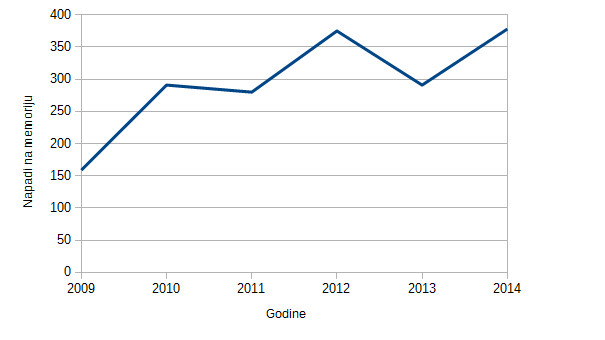
\includegraphics[width=12cm, height=8cm]{slike/memory_corruption}
\caption{Graf napada na memoriju u razdoblju 2009-2014}
\label{fig:mem_corruption} 
\end{figure} 

\section{Preljev Spremnika}
\label{sct:bufferOverflow}

Preljev spremnika je oblik ranjivosti u kojemu se podaci upisuju
u spremnik van njegovih granica. Do preljeva spremnika dolazi
kada program pokušava upisati podatke u polje fiksne veličine,
pri čemu je veličina podataka koji se žele upisati veća od
veličine polja. Posljedica toga je što susjedne memorijske
lokacije, koje ne pripadaju ranjivom spremniku, sadrže podatke
koji mogu izazvati ne definirano ponašanje programa. Ranjivost
preljeva spremnika moguće je iskoristit kada napadači žele
izvršiti neki strani programski kod ili kako bi se promijenio
način na koji program radi. 

Programski jezici koji se najčešće spominju u kontekstu preljeva
spremnika su C i C++. Razlog tome je što navedeni programski
jezici nemaju ugrađeni oblik zaštite koji bi kontrolirao
upisivanje podataka na bilo koje mjesto u memoriji. Također, C i
C++ nemaju automatski način provjere podataka u smislu da podaci
koji se upisuju u spremnik budu unutar njegovih granica.

Preljev spremnika može se podijeliti u dvije kategorije koje su
opisane u nastavku:

\begin{enumerate}
\item Preljev spremnika na stogu
\item Preljev spremnika na gomili
\end{enumerate}

\subsection{Preljev Spremnika na Stogu}

Preljev spremnika na stogu može se iskoristiti na nekoliko
načina:

\begin{itemize}
\item prepisati vrijednost lokalne varijable koja se nalazi blizu
ranjivog spremnika čime je moguće promijeniti ponašanje programa
\item prepisati vrijednost povratne adrese. Na taj način napadač
je u mogućnosti prebaciti izvršavanje programa na neki strani
kod. Ovaj način preljeva detaljno je prikazan u nastavku.
\item prepisati vrijednost pokazivača na funkcije. Na taj način
moguće je prepisati pokazivač za funkciju zaduženu za rukovanje
iznimkama čime se izvršavanje ponovno prebacuje na neki strani
kod.
\end{itemize}

Glavni cilj napadača, prilikom iskorištavanja preljeva spremnika
na stogu, je prepisati povratnu adresu. U nastavku je dan primjer
ranjivog programskog koda sa detaljnim objašnjenjem.

\begin{lstlisting}[frame=single, caption=Primjer preljeva spremnika na stogu, label={lst:stackBuffOverflow}]
#include <string.h>
 
void funkcija (char *arg)
{
   char  c[12];
 
   strcpy(c, arg);  // no bounds checking
}
 
int main (int argc, char **argv)
{
   foo(argv[1]);
}
\end{lstlisting}

Programski kod u odsječku \ref{lst:stackBuffOverflow} radit će
sasvim normalno za znakovne nizove manje od 12 znakova. Na slici
\ref{fig:buff_overflow_nodata} i slici
\ref{fig:buff_overflow_legitdata} prikazan je izgled stoga prije
kopiranja te prilikom kopiranja znakovnog niza koji zadovoljava
granice.

\pagebreak
\begin{figure}[!ht]
\centering
\setlength\fboxsep{0pt}
\setlength\fboxrule{0.5pt}
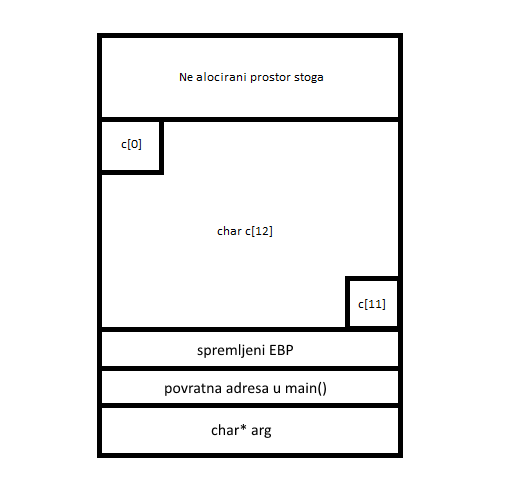
\includegraphics[width=12cm, height=10cm]{slike/buffer_overflow_nodata}
\caption{Primjer stoga prije kopiranja podataka}
\label{fig:buff_overflow_nodata} 
\end{figure} 

\begin{figure}[!ht]
\centering
\setlength\fboxsep{0pt}
\setlength\fboxrule{0.5pt}
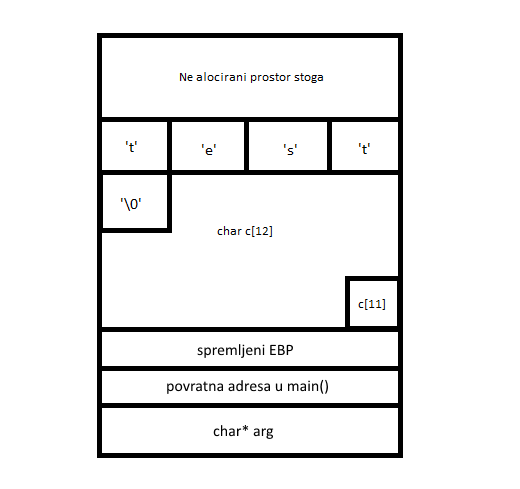
\includegraphics[width=12cm, height=10cm]{slike/buffer_overflow_legitdata}
\caption{Primjer stoga nakon kopiranja znakovnog niza "test"}
\label{fig:buff_overflow_legitdata} 
\end{figure} 
\pagebreak

Na slici \ref{fig:buff_overflow_overflow} prikazan je izgleda
stoga nakon što je kao argument programu predan znakovni niz
"AAAAAAAAAAAAAAAA0835C080" pri čemu adresa \emph{0x80C03508}
pokazuje na početak lokalne varijable \emph{c} unutar funkcije.
Ukoliko se sada izvrši \emph{ret} instrukcija, program će
nastaviti s izvršavanjem od adrese \emph{0x80C03508} koja u ovom
slučaju sadrži nepravilne vrijednosti ("AA.."). Jasno je kako je
umjesto znakovnog niza "AAA..." mogao biti predan operacijski kod
legitimnih instrukcija procesora koje bi bile u mogućnosti
izvršiti zadatke koji se od programa u primjeru ne očekuju.

\begin{figure}[!ht]
\centering
\setlength\fboxsep{0pt}
\setlength\fboxrule{0.5pt}
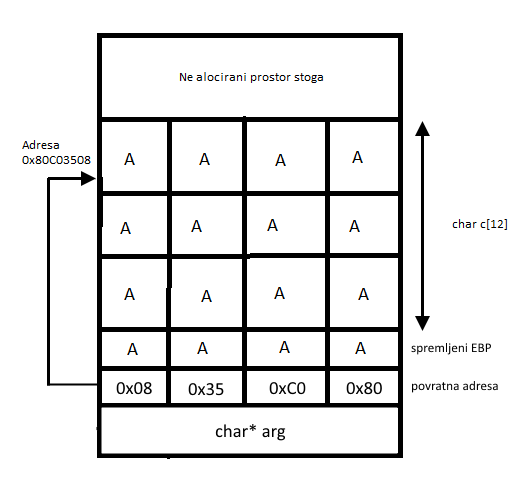
\includegraphics[width=12cm, height=10cm]{slike/buffer_overflow_overflow}
\caption{Primjer stoga nakon kopiranja znakovnog niza koji uzrokuje preljev}
\label{fig:buff_overflow_overflow} 
\end{figure}

Ovo je dobar trenutak za objasniti kako DEP(\ref{sct:dep})
sprječava izvršavanje ubačenog programskog koda. Ukoliko je DEP
aktiviran u ovome primjeru, prilikom izvršavanja \emph{ret}
instrukcije i skoka na adresu \emph{0x80C03508} program će se
zaustaviti jer DEP onemogučava izvršavanje instrukcija na stogu,
tj. upotrebom DEP-a sve memorijske lokacije na stogu postavljene
su kao ne izvršne. Iz tog razloga napadači se trebaju poslužiti
drugim metodama kako bi iskoristili ranjivost preljeva spremnika
na stogu. Više o toj temi u poglavlju \ref{sct:rop}.

\subsection{Preljev Spremnika na Gomili}
\label{scr:heap_overflow}

U ovom poglavlju ukratko je opisana arhitektura gomile unutar
Microsoft Windows operacijskog sustava te je prikazano kako je
moguće iskoristiti ranjivost preljeva spremnika na gomili.

Gomila je dio memorije čiji dijelovi se mogu dinamički alocirati
prilikom izvršavanja programa. Preljev spremnika na gomili
iskorištava se na drugačiji način nego preljev spremnika na
stogu. Razlog tome je što se kod iskorištavanja korupcije
memorije unutar gomile, obavlja prepisivanje određenih internih
podatkovnih struktura poput pokazivača povezane liste.

Svaki proces, prilikom kreiranja, dobiva gomilu. Početna veličina
dobivene gomile je 1MB te ista može rasti ukoliko za to postoji
potreba. Maksimalna veličina gomile određena je količinom
memorije u sustavu. Također, valja napomenuti kako svaki proces
može stvarati i dodatne, privatne gomile pomoću WIN32 API
funkcija \emph{HeapCreate()/HeapDestroy()}. Jednom kada su
privatne gomile stvorene moguće ih je koristiti preko API
funkcija \emph{HeapAlloc()/HeapFree()}.

\subsubsection{Indexi}
Osnovna građevna jedinica svake gomile su blokovi veličine 8
okteta koji se nazivaju \emph{indexi}. Posljedica toga je što
svaki puta kada proces alocira prostor na gomili, on dobiva na
korištenje blokove čija veličina je višekratnik od 8, tj. dobiva
na korištenje određen broj \emph{indexa}. Za primjer, ukoliko
proces želi alocirati blok memorije veličine 32 okteta, njemu se
vračaju 4 \emph{indexa}. Važno za naglasiti je kako se alocirani
blokovi zauzimaju slijedno, tj. jedan iza drugoga kako je
prikazano na slici \ref{fig:heap_2_allocated_blocks}.

\begin{figure}[!ht]
\centering
\setlength\fboxsep{0pt}
\setlength\fboxrule{0.5pt}
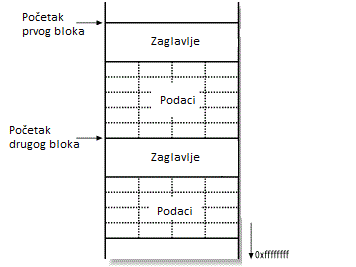
\includegraphics[width=8cm, height=8cm]{slike/heap_2_allocated_blocks}
\caption{Primjer dva bloka unutar gomile}
\label{fig:heap_2_allocated_blocks} 
\end{figure}

Kako bi se što jednostavnije upravljalo alociranim blokovima
memorije, stvoreno je i posebno zaglavlje za svaki memorijski
blok. Navedeno zaglavlje je također veličine koja je višekratnik
broja 8 te iznosi 16 okteta. Valja napomenuti kako zaglavlje
postoji u dva oblika kao što je i prikazano na slikama
\ref{fig:used_heap_block} i \ref{fig:free_heap_block}. U
konačnici, ukupna količina memorije koja se alocira jednaka je
traženoj veličini uvečanoj za veličinu zaglavlja.

\pagebreak

\begin{figure}[!ht]
\centering
\setlength\fboxsep{0pt}
\setlength\fboxrule{0.5pt}
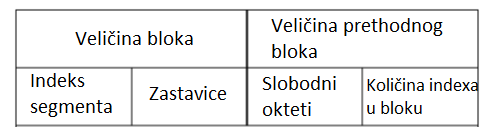
\includegraphics[width=11cm, height=3cm]{slike/used_heap_block}
\caption{Zaglavlje korištenog memorijskog bloka}
\label{fig:used_heap_block} 
\end{figure}

\begin{figure}[!ht]
\centering
\setlength\fboxsep{0pt}
\setlength\fboxrule{0.5pt}
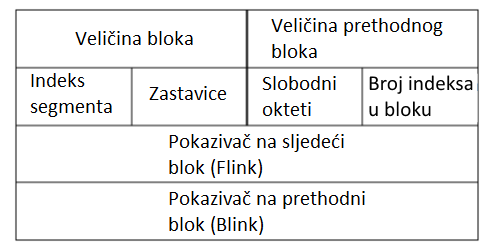
\includegraphics[width=11cm, height=5cm]{slike/free_heap_block}
\caption{Zaglavlje slobodnog memorijskog bloka}
\label{fig:free_heap_block} 
\end{figure}
\pagebreak

Svako zaglavlje sastoji se od sljedećih elemenata:

\begin{itemize}
\item Veličina bloka: Ukupna veličina bloka memorije (uključujući i zaglavlje)
\item Veličina prethodnog bloka: Ukupna veličina bloka koji se nalazi prije promatranoga. Također uključuje i veličinu zaglavlja.
\item Indeks segmenta: Indeks segmenta u memoriji unutar kojega se blok nalazi.
\item Zastavice: Opisuju određena svojstva blokova u pripadajućoj gomili.
\item Slobodni okteti: Broj slobodnih okteta u bloku.
\item Količina \emph{indexa} u bloku: Sadrži broj \emph{indexa} od kojih se blok sastoji. 
\item Flink: Koristi se samo kod slobodnih blokova. Pokazuje na sljedeći slobodni blok u dvostruko povezanoj listi.
\item Blink: Koristi se samo kod slobodnih blokova. Pokazuje na prethodni slobodni blok u dvostruko povezanoj listi.
\end{itemize}

\subsubsection{Arhitektura Gomile}

Svaka gomila započinje strukturom prikazanom na slici
\ref{fig:heap_structure}. Iako navedena struktura sadrži dosta
elemenata, za potrebe opisivanja preljeva spremnika na gomili
važno je uočiti element na pomaku \emph{0x178} unutar strukture.
Radi se o polju (\emph{FreeLists}) koje sadrži 128 elemenata
\emph{LIST\_ENTRY} strukture. Svaka \emph{LIST\_ENTRY} struktura
sadrži dva pokazivača kao što je prikazano na odsječku koda
\ref{lst:list_entry_struct}.

\begin{lstlisting}[frame=single, caption=LIST\_ENTRY struktura, label={lst:list_entry_struct}]
typedef struct _LIST_ENTRY {
  struct _LIST_ENTRY  *Flink;
  struct _LIST_ENTRY  *Blink;
} LIST_ENTRY, *PLIST_ENTRY;
\end{lstlisting}

Pokazivači unutar \emph{LIST\_ENTRY} strukture imaju sljedeće vrijednosti:

\begin{itemize}
\item \emph{Flink}: Pokazuje na sljedeći element liste ili početak liste ukoliko ne postoji sljedeći element.
\item \emph{Blink}: Pokazuje na prethodni element liste ili na početak liste ukoliko je lista prazna.
\end{itemize}

\begin{figure}[!ht]
\centering
\setlength\fboxsep{0pt}
\setlength\fboxrule{0.5pt}
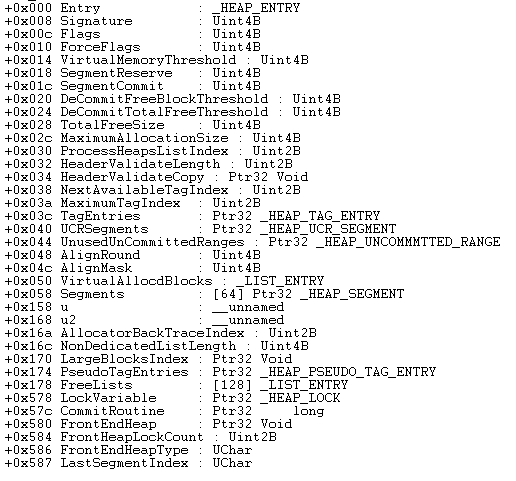
\includegraphics[width=12cm, height=10cm]{slike/heap_structure}
\caption{Osnovna struktura gomile}
\label{fig:heap_structure} 
\end{figure}

\emph{FreeLists} struktura sadrži pokazivače na slobodne blokove
unutar gomile. Svaki puta kada se neki memorijski blok dealocira,
on se premješta na odgovarajuće mjesto unutar \emph{FreeLists}
strukture. Ovdje do izražaja dolazi količina \emph{indexa} koji
sačinjavaju pojedini blok. Naime, upravo količina \emph{indexa} u
bloku određuje kojem indeksu unutar \emph{FreeLists} strukture će
se pojedini blok dodijeliti jednom kada bude slobodan. Za
primjer, ukoliko neki blok sadrži 192 okteta (24 \emph{indexa})
on će se prilikom oslobađanja pohraniti u listu pod indeksom
\emph{FreeLists[24]}. Valja još napomenuti par graničnih
vrijednosti:

\begin{itemize}

\item Polje \emph{FreeLists[0]} koristi se za blokove koji su
veći od 127 \emph{indexa}, tj. blokovi veći od 1016 okteta.

\item Polje \emph{FreeLists[1]} se ne koristi jer je nemoguće da
blok sadrži samo 8 okteta tj. samo jedan \emph{index}.

\end{itemize}

U trenutku kada je gomila stvorena, pokazivač na indeksu 0 iz
\emph{FreeLists} polja pokazuju na prvi slobodni blok. Primjera
radi, ako je gomila stvorena na adresi \emph{0x00350000} tada se
prvi slobodni blok može nalaziti na adresi \emph{0x00350688}.
Navedeno je prikazano na odsječku koda \ref{lst:freeLists0}.

\begin{lstlisting}[frame=single, caption=Prvi slobodni blok gomile, label={lst:freeLists0}]
0x00350178 (FreeList[0].Flink) = 0x00350688 (Prvi Slobodni Blok)
0x0035017C (FreeList[0].Blink) = 0x00350688 (Prvi Slobodni Blok)

0x00350688 (Prvi Slobodni Blok) = 0x00350178 (FreeList[0])
0x0035068C (Prvi Slobodni Blok+4) = 0x00350178 (FreeList[0])
\end{lstlisting}

Način na koji je organizirano \emph{FreeLists} polje struktura
prikazan je na slici \ref{fig:free_lists_entries}.

\begin{figure}[!ht]
\centering
\setlength\fboxsep{0pt}
\setlength\fboxrule{0.5pt}
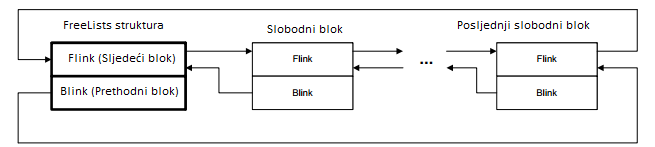
\includegraphics[width=15cm, height=4cm]{slike/free_lists_entries}
\caption{Dvostruko-povezana lista slobodnih blokova}
\label{fig:free_lists_entries} 
\end{figure}

\subsubsection{Preljev Gomile}

Sada kada je objašnjen način na koji funkcionira gomila unutar
Windows operacijskog sustava, iskoristit ćemo jednostavan primjer
kako bi prikazali preljev spremnika na gomili.

Unutar odsječka koda \ref{lst:heapOverflowExmp} nalazi se ranjiva
funkcija unutar koje je moguće izazvati preljev spremnika na
gomili. U nastavku slijedi detaljan opis funkcije.

\begin{lstlisting}[frame=single, caption=Primjer preljeva gomile, label={lst:heapOverflowExmp}]
DWORD vulner(LPVOID str)
{
    HANDLE h = HeapCreate(0, 0, 0);
 
    LPVOID m1 = HeapAlloc(h, 0 , 64);
    LPVOID m2 = HeapAlloc(h, 0,128);
 
    HeapFree(m2);

    memcpy((char *)m1, 0x31, 64+16);
 
    m2 = HeapAlloc(h, 0, 128);
 
    return 0;
}
\end{lstlisting}

U početku su alocirana dva memorijska bloka na gomili te su, kao
što je ranije spomenuto, pozicionirani slijedno
(\ref{fig:heap_2_allocated_blocks}). Na liniji 8 vidljivo je kako
se blok \emph{m2} oslobađa te se informacije o bloku pohranjuju u
odgovarajući indeks unutar \emph{FreeLists} strukture.	Na liniji
10 događa se postupak preljeva, tj. memorijski blok \emph{m1} se
cijeli popunjava te uz njega i zaglavlje slobodnog memorijskog
bloka \emph{m2}.

U ovome trenutku, pokazivači \emph{Flink} i \emph{Blink} unutar
zaglavlja bloka \emph{m2} su prepisani, tj. postavljeni su na
proizvoljne vrijednosti napadača.

Na liniji 12 nalazi se ključan dio koda koji omogućava
iskorištavanje preljeva spremnika na gomili. Naime, nakon što se
ponovno alocira blok veličine 128 okteta potrebno je isti taj
blok maknuti iz \emph{FreeLists} polja jer on više nije slobodan.
Način na koji se to obavlja je sljedeći:

\begin{enumerate}

\item \emph{Blink} pokazivač sljedećeg slobodnog bloka
(\emph{m2->Flink}) potrebno je postaviti tako da pokazuje na
prethodni slobodni blok (\emph{m2->Blink}). Pošto su polja
\emph{Flink} i \emph{Blink} bloka \emph{m2} prepisana, događa se
upisivanje proizvoljne vrijednosti (vrijednost \emph{m2->Blink})
na proizvoljnu lokaciju (\emph{m2->Flink}).

\item \emph{Flink} pokazivač prethodnog elementa
(\emph{m2->Blink}) potrebno je postaviti tako da pokazuje na
sljedeći slobodni blok (\emph{m2->Flink}). Ovdje se ponovno
događa situacija kao i u koraku 1, tj. ponovno se obavlja pisanje
proizvoljne vrijednosti na proizvoljnu memorijsku lokaciju.

\end{enumerate}

Ono što je napadaču najvažnije u ovome postupku je što se
događaju dvije operacije pisanja u memoriju. Iz tog razloga
napadač može preljevom spremnika kontrolirati koja vrijednost će
se upisati i gdje. Na primjer, moguće je prepisati pokazivač na
funkciju destruktora nekog objekta na način da isti pokazuje na
strani, ubačeni kod.

\section{Napad Format Znakovnim Nizom}

Napad format znakovnim nizom (engl. \emph{Format String Attack})
jedan je od starijih načina kako iskoristiti korupciju memorije.
Ova ranjivost najčešće se iskorištava u sustavima gdje ne postoji
provjera ulaznih podataka od strane korisnika te gdje se ti isti
podaci mogu interpretirati kao naredbe. Iz tog razloga napadač je
u mogućnosti izvršiti strani kod, čitati podatke sa stoga ili
izazvati rušenje programa. 

Kako bi ovaj oblik ranjivosti bio jasniji, u nastavku su opisani
pojedini dijelovi potrebni za uspješno iskorištavanje format
nizova:

\begin{itemize}
\item Format funkcija: Radi se o funkcijama karakterističnima za
C i C++ programske jezike. Navedene funkcije primaju proizvoljan
broj argumenata te pretvaraju te argumente (ovisno o njihovom
tipu) u znakovni niz. Neke od tipičnih format funkcija su:
\emph{printf(), fprintf(),...}. 

\item Format znakovni niz: Format znakovni niz je običan ASCII
znakovni niz koji sadrži tekst i parametre formata. Predaje se
kao argument Format funkcijama kako bi iste mogle procesirati
razne vrste argumenata koje je potrebno prikazati kao znakovni
niz. Primjer format znakovnog niza je sljedeći:
\emph{printf("Ispis broja \%d", 88)}.

\item Format parametri: Označavaju način kako obraditi argumente
format funkcije i prikazati ih kao znakovni niz. Najčešće
korišteni format parametri vidljivi su u tablici
\ref{tbl:format_parameters}.
\end{itemize}

Kao što je već spomenuto, ovaj oblik napada najčešće se događa
ukoliko napadnuta aplikacija ne provjerava ulazne podatke koji se
prenose kao parametri format funkcijama. Na primjer, ukoliko je
format parametar poput \emph{\%x} ubačen u ulazne podatke te
predan sa podacima format funkciji, ista će interpretirati
navedeni parametar te izvršiti konverziju specificiranu
parametrom. Ako u tom slučaju nema dodatnih argumenata funkciji,
ista će obaviti nedozvoljeno čitanje sa stoga. Na taj način
moguće je stvoriti veće i opasnije format znakovne nizove koji bi
u konačnici mogli srušiti program ili izvršiti strani kod.

Najčešće korišteni format parametri koji se koriste prilikom
iskorištavanja ove ranjivosti su:

\begin{itemize}
\item \emph{\%x}: Čita podatke sa stoga u heksadecimalnom zapisu.
\item \emph{\%s}: Čita znakovni niz iz memorije.
\item \emph{\%n}: Upisuje cjelobrojnu varijablu u memoriju. 
\end{itemize}

U tablici \ref{tbl:format_parameters} prikazani su i ostali
format parametri koji se također mogu predati format funkcijama
kako bi se ustanovilo postoji li ranjivost.

\begin{table}[htb]
\small
\caption{Parametri korišteni kod napada format znakovnim nizom}
\label{tbl:format_parameters}
\centering
\begin{tabular}{|l|p{8cm}|}
\hline
Parametar & Izlaz \\ \hline
\%p & Opis pokazivača na \emph{void} tip podataka \\ \hline
\%d & Opis cjelobrojnog tipa podataka \\ \hline
\%c & Opis jednog znaka \\ \hline
\%u & Opis pozitivnog cjelobrojnog podatka \\ \hline
\end{tabular}
\end{table}

Kako bi poglavlje o napadu format znakovnim nizom bilo kompletno,
u nastavku je prikazan primjer ranjivog programa te kako se isti
ponaša prilikom predaje raznih argumenata format funkciji.

U odsječku koda \ref{lst:formatStringExmp} prikazan je ranjivi
program. Ranjivost je očita jer se ulazni parametar programa
jednostavno kopira u polje \emph{buffer} koje se zatim predaje
format funkciji \emph{printf()}. 

\begin{lstlisting}[frame=single, caption=Primjer ranjivog programa, label={lst:formatStringExmp}]
#include  <stdio.h>
#include  <string.h>
#include  <stdlib.h>

#include<stdio.h>
int main(int argc, char** argv) {
	char buffer[100];
	strncpy(buffer, argv[1], 100);
	printf(buffer);
	return 0;
}
\end{lstlisting}

Prikazanu ranjivost moguće je iskoristit na nekoliko načina.
Ukoliko se kao argument preda niz \emph{"\%x \%x \%x \%x \%x \%x
\%x \%x \%x"}, funkcija će očekivati još devet parametara na
stogu te će se obaviti čitanje sa stoga. Ukoliko su na stogu u
datom trenutku pohranjeni neki važni podaci, napadač može iste
pročitati te u konačnici ugroziti cijeli sustav. Primjer ispisa
za navedeni ulaz prikazan je u odsječku koda
\ref{lst:formatStringStackRead}.

\begin{lstlisting}[frame=single, caption=Primjer rada program, label={lst:formatStringStackRead}]
./program "%x%x%x%x%x%x%x%x%x"

0 0 7ffda000 cccccccc cccccccc cccccccc cccccccc cccccccc cccccccc
\end{lstlisting}

Drugi način na koji je moguće iskoristiti danu ranjivost je
izazivanje prekida rada programa. Ukoliko se kao argument
programu preda niz \emph{"\%s \%s \%s \%s"} doći će prekida rada.
Razlog tome je što format parametar \emph{\%s} čita adresu sa
stoga te istu interpretira kao pokazivač na znakovni niz u
memoriju. Ukoliko je ta adresa nepravilna ili pokazuje na
nedozvoljeni prostor u memoriji doći će do prekida rada programa.

\section{Napad Dodatnom \emph{free()} Metodom}

Do napada dodatnom \emph{free()} metodom (engl. \emph{Double Free
Attack}) dolazi ukoliko se \emph{free()} funkcija poziva više
puta sa istim blokom memorije kao argumentom. Kao posljedica,
dolazi do korupcije podatkovnih struktura u memoriji čime se
napadaču omogućava upisivanje proizvoljnih vrijednosti na
proizvoljne memorijske lokacije. Navedena ranjivost može
uzrokovati prestanak rada programa ili promjene u toku
izvršavanja. Također, ovaj oblik ranjivosti usko je povezan sa
preljevom gomile jer se prepisuju iste podatkovne strukture za
upravljanje memorijom.

Pošto je većina informacija o detaljima ove ranjivosti ispričana
u poglavlju o preljevu gomile \ref{scr:heap_overflow}, u nastavku
je samo dan primjer kako se navedena ranjivost mogla iskoristiti.

Kao što je već navedeno, prilikom oslobađanja bloka memorije na
gomili isti se ubacuje u dvostruko povezanu listu slobodnih
blokova. Ukoliko se nad istim blokom ponovno proba pozvati
\emph{free()} metoda, isti će blok ponovno završiti u listi
slobodnih blokova. Znači, pokazivač na isti blok memorije
pojavljuje se u listi slobodnih blokova dva puta.

U sljedećem koraku ukoliko se navedeni blok ponovno proba
alocirati, dogoditi će se to što će isti blok memorije postojati
u dva stanja: alociranom i nealociranom. Problem koji se ovdje
javlja je što sada napadač ima kontrolu nad pokazivačem na blok
koji se još uvijek nalazi u listi slobodnih blokova. Na taj način
moguće je prepisati internu strukturu (pokazivače \emph{Flink} i
\emph{Blink}). Posljednji korak je alociranje bloka koji se još
uvijek nalazi u listi slobodnih blokova pri čemu se, kao i kod
preljeva gomile, događa upisivanje proizvoljnih vrijednosti na
proizvoljne adrese. Navedeno je prikazano na slici
\ref{fig:double_free}.

\begin{figure}[!ht]
\centering
\setlength\fboxsep{0pt}
\setlength\fboxrule{0.5pt}
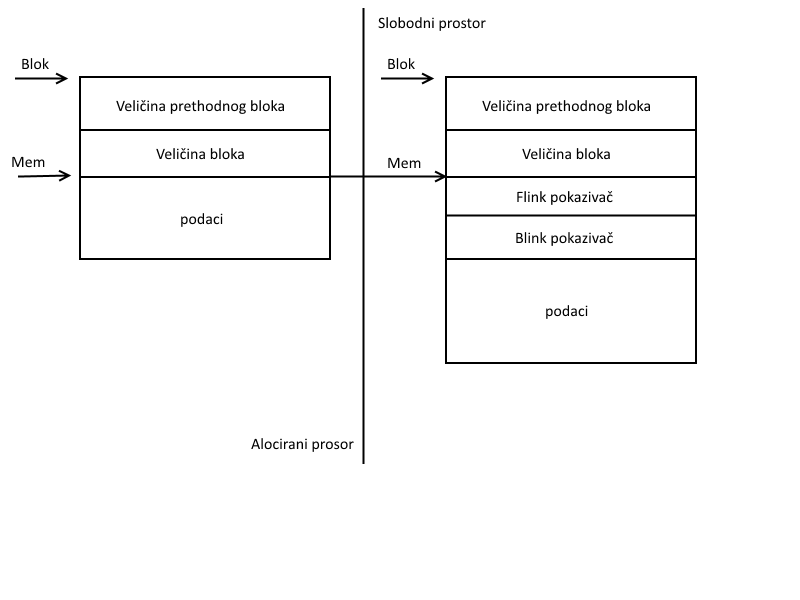
\includegraphics[width=15cm, height=10cm]{slike/double_free}
\caption{Stanje gomile kod dvostruke \emph{free()} metode}
\label{fig:double_free} 
\end{figure}

\pagebreak
 
\section{Programiranje Temeljeno na "ret" Blokovima}
\label{sct:rop}

Cilj ovog poglavlja je upoznati čitatelja sa novijom i danas
najraširenijom metodom iskorištavanja propusta vezanih za
korupciju memorije. Osim detaljno opisanog načina kako ovaj oblik
napada radi, u sklopu poglavlja se nalazi i nekoliko primjera
pomoću kojih bi metoda trebala biti jednostavnija za shvatiti.
Također, u poglavlju je opisano i koje metode zaštite protiv
navedenog napada danas postoje te kako bi modul za promjenu koda
dodatno unaprijedio postojeće mehanizme zaštite.

Programiranje temeljeno na "ret" blokovima (engl. \emph{Return
Oriented Programming}) je tehnika koja se prvi puta spominje
2007. u istoimenom članku \citep{rop_official}. Ovaj oblik
iskorištavanja ranjivosti vezanih za korupciju memorije omogućava
napadaču da preuzme kontrolu nad programom čak i u sustavima u
kojima je aktivan ranije spomenuti mehanizam zaštite - DEP
\ref{sct:dep}. Štoviše, ova tehnika razvijena je upravo kao
protuteža spomenutom mehanizmu zaštite.

Kako bi se programiranje temeljeno na "ret" blokovima uopće moglo
upotrijebiti, nužno je da program čiji se sigurnosni propust
iskorištava bude ranjiv na metodu preljeva spremnika. Kao što je
spomenuto u ranijem poglavlju \ref{sct:bufferOverflow}, postupak
iskorištavanja preljeva spremnika može se podijeliti u 3 koraka:

\begin{enumerate}
\item Korak: Prekoračiti granice lokalne varijable. Time dolazi
do prepisivanja povratne adrese.
\item Korak: Prouzročiti da preljev bude takav da se povratna
adresa prepiše vrijednošću na kojoj se nalazi strani, ubačeni
kod. Time se u trenutku povratka iz funkcije, preuzima kontrola
nad EIP registrom, tj. isti sadrži adresu ubačenog koda od strane
napadača.
\item Korak: Ubačeni kod može se nalaziti na stogu ili na gomili
te ga je moguće izvršiti nakon što je preuzeta kontrola nad EIP
registrom.
\end{enumerate}

Gore opisani koraci vrijediti će ukoliko na sustavu nije aktivan
DEP. Međutim, ukoliko je DEP aktiviran, doći će do prekida rada
programa u koraku 3 jer su stog i gomila označeni kao memorijski
prostor unutar kojega nije moguće izvršavanje!

Upravo iz toga razloga se pojavila potreba za programiranjem
zasnovanim na "ret" blokovima. Glavna ideja ove vrste
iskorištavanja sigurnosnih propusta je upotreba već postojećih
dijelova programskog koda. Ti postojeći dijelovi programskog koda
(u nastavku teksta nazivaju se \emph{blokovi}) izgrađeni su od
nekoliko instrukcija pri čemu posljednja instrukcija u bloku mora
biti "ret". Iz tog razloga moguće je povezivanjem više manjih
"ret" blokova, gdje svaki blok obavlja određenu zadaću,
konstruirati složene operacije pri čemu se u potpunosti gubi
potreba za ubacivanjem stranog koda od strane napadača. Spomenute
"ret" blokove moguće je stoga pronaći unutar samog programa čija
ranjivost se iskorištava ili unutar dijeljenih biblioteka.

Prije nego se krene u detaljno objašnjenje primjera koji
prikazuje kako programiranje temeljeno na "ret" blokovima radi,
potrebno je ukratko opisati metodu koja se smatra pretečom ovog
oblika napada.

\subsection{Napad \emph{ret2lib}}

Napad ret2lib prvi puta se pojavio još 1997. godine
\citep{ret2lib_official} i smatra se pretečom programiranju
zasnovanom na "ret" blokovima. Glavna ideja ovog napada je ta da
se tok programa nakon uspješno izvedenog preljeva spremnika na
stogu, prebaci na već postojeću funkciju. Funkcija koja se pritom
najčešće pozivala je \emph{system('/bin/sh')} pošto se ista
nalazi unutar \emph{libc} biblioteke koja je povezana sa većinom
pokrenutih programa u sustavu.

Kako bi navedeni napad funkcionirao, potrebno je stvoriti lažni
okvir funkcije na stogu. To je potrebno iz razloga što
\emph{system()} funkcija mora imati svoj okvir stoga sa kojega
može čitati parametre te na kojemu se nalazi povratna adresa
nakon što funkcija završi s izvođenjem. Na odsječku koda
\ref{lst:stackBuffOverflow_ret2lib} prikazana je funkcija ranjiva
na napad preljeva spremnika na stogu.

\begin{lstlisting}[frame=single, caption=Primjer preljeva spremnika na stogu, label={lst:stackBuffOverflow_ret2lib}]
#include <string.h>
 
void func1 (char *s)
{
	char buffer[80];
	strcpy(buffer, s);
}

\end{lstlisting}

Na slici \ref{fig:ret2lib_stackFrame} prikazan je izgled okvira
stoga za tu funkciju, dok je na slici \ref{fig:ret2lib} prikazana
situacija kada se dogodi preljev spremnika na stogu. Kod ovog
primjera preljeva spremnika, povratna adresa prepisana je adresom
\emph{system()} funkcije te je na stog zapisan i lažni okvir kako
bi se \emph{system()} funkcija mogla izvršiti.  

\pagebreak

\begin{figure}[!htb]
\centering
\setlength\fboxsep{0pt}
\setlength\fboxrule{0.5pt}
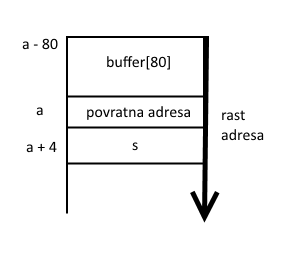
\includegraphics[width=5cm, height=5cm]{slike/ret2lib_stackFrame}
\caption{Izgled stoga za funkciju \emph{func1(char *s)}}
\label{fig:ret2lib_stackFrame} 
\end{figure}

\begin{figure}[!htb]
\centering
\setlength\fboxsep{0pt}
\setlength\fboxrule{0.5pt}
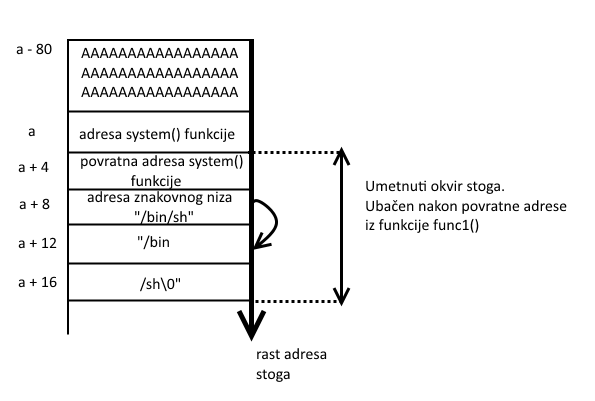
\includegraphics[width=13cm, height=12cm]{slike/ret2lib}
\caption{Izgled stoga za funkciju \emph{func1(char *s)} nakon preljeva spremnika}
\label{fig:ret2lib} 
\end{figure}

Ukoliko dođe do situacije prikazane na slici \ref{fig:ret2lib},
nakon što funkcija \emph{func1()} završi s izvršavanjem, u
registar EIP upisati će se adresa \emph{system()} funkcije te će
se izvršavanje programa nastaviti od tamo. U tom trenutku na
stogu će postojati legitiman okvir (lažni) gdje će biti podaci o
parametrima te o povratnoj adresi iz \emph{system()} funkcije
koju opet kontrolira napadač. Valja uočiti kako napadač ima
kontrolu nad EIP registrom i nakon što \emph{system()} funkcija
završi sa svojim radom. Na taj način moguće je stvoriti dodatne
lažne okvire stoga koji će se slijedno pozivati te u konačnici
obaviti neku složenu operaciju. 

\subsection{Programiranje sa "ret" Blokovima}
\label{sct:rop2}

U prethodnom poglavlju dan je kratak uvod u \emph{ret2lib}
napade. Programiranje sa "ret" blokovima je zapravo jedan oblik
\emph{ret2lib} napada. Radi se o tome što je programiranje "ret"
blokovima zapravo generalizirajući slučaj \emph{ret2lib} napada,
tj. dok se \emph{ret2lib} napad orijentira na poziv funkcija iz
dijeljenih biblioteka, programiranje temeljeno na "ret" blokovima
pretpostavlja kako se bilo koji dio ranjivog programa ili
dijeljene biblioteke može iskoristiti za obavljanje pojedinih
zadaća sve dok taj dio (blok koda) završava sa \emph{ret}
instrukcijom. Te blokove je moguće povezivati kako bi tvorili
smislene cjeline koje u konačnici mogu obaviti i zahtjevnije
računarske operacije.

Prije nego se krene u detaljan opis programiranja temeljenog na
"ret" blokovima, potrebno  je spomenuti konvencije poziva
funkcija. Konvencije poziva funkcija definiraju način na koji se
funkcije pozivaju u programu, tj. preko njih se definira kako se
parametri prenose funkciji te kako je organiziran stog pojedine
funkcije. U nastavku su navedene i ukratko opisane tri
najpoznatije konvencije poziva:

\begin{itemize}

\item \emph{cdecl} konvencija poziva: Radi se o standardnoj
konvenciji poziva za C i C++ programske jezike. Glavna
karakteristika ove konvencije je što pozivatelj funkcije čisti
stog od argumenata nakon što funkcija završi s izvršavanjem. Svi
parametri se funkciji prenose putem stoga.

\item \emph{fastcall} konvencija poziva: Ova konvencija ima bolje
performanse od preostale dvije. Razlog tome je što koristi
registre procesora za prijenos argumenata funkciji. Konkretno,
koristi registre ECX i EDX za prijenos prva dva argumenta dok se
ostatak argumenata prenosi pute stoga. Ovu konvenciju danas
koristi većina prevoditelja (engl. \emph{compiler}).

\item \emph{stdcall} konvencija poziva: Za potrebe ovog rada ovo
je najvažnija konvencija poziva jer se ista koristi u većini
funkcija Windows API-a. Navedena konvencija dosta je slična
\emph{cdecl} konvenciji s razlikom što sama funkcija čisti stog
od argumenata. Navedena funkcionalnost ostvarena je pomoću
\emph{RET} instrukcije kojoj je moguće predati dodatni parametar
koji označava koliko argumenata je potrebno ukloniti sa stoga.
\end{itemize}

Na odsječku koda \ref{lst:rop_example} prikazan je primjer
programa na kojemu je u nastavku prikazan način iskorištavanja
ranjivosti pomoću programiranja temeljenog na "ret" blokovima.
Glavna ideja je da se preko ranjivosti preljeva spremnika u
funkciji \emph{func1()} ubaci lažni okvir stoga čime će se
pozvati funkcija \emph{add()} sa parametrima 5 i 6.
 
\begin{lstlisting}[frame=single, caption=Primjera programa za
programiranje "ret" blokovima, label={lst:rop_example}]
#include <string.h>
 
void func1 (char *s) { char buffer[80]; strcpy(buffer, s); }

void add (int x, int y)
{
	int sum;
	sum = x + y;
	printf("%d\n", sum);
}

int main(int argc, char *argv)
{
	add(3,4);
	func1(argv[1]);
}
\end{lstlisting}
Izgled stoga prilikom poziva funkcije \emph{add(3,4)} prikazan je na slici \ref{fig:rop_add34} dok je za funkciju \emph{func1()} prikazan na slici \ref{fig:ret2lib_stackFrame}.

\begin{figure}[!htb]
\centering
\setlength\fboxsep{0pt}
\setlength\fboxrule{0.5pt}
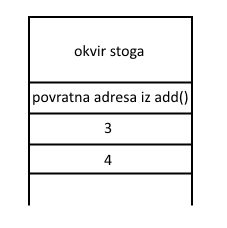
\includegraphics[width=5cm, height=5cm]{slike/rop_add34}
\caption{Izgled stoga za funkciju \emph{add(3,4)}}
\label{fig:rop_add34} 
\end{figure}
Kako bi se preko \emph{func1()} funkcije mogla pozvati funkcija \emph{add(5,6)} potrebno je učiniti sljedeće:
\begin{itemize}
\item Izazvati preljev spremnika u funkciji \emph{func1()} tako da se povratna adresa prepiše adresom funkcije \emph{add()}. Adresu funkcije \emph{add()} moguće je jednostavno naći unutar \emph{debugger} programa ukoliko nije aktivan mehanizam zaštite ASLR\ref{sct:aslr}.
\item Uz prepisivanje povratne adrese, potrebno je na stog postaviti i lažni okvir stoga za funkciju \emph{add(5,6)} koju želimo pozvati.
\end{itemize}
U konačnici stog bi trebao izgledati kako je prikazano na slici \ref{fig:rop_add56}.

\begin{figure}[!htb]
\centering
\setlength\fboxsep{0pt}
\setlength\fboxrule{0.5pt}
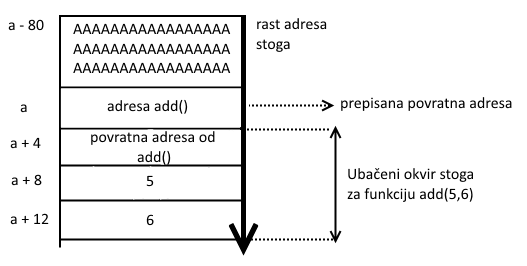
\includegraphics[width=10cm, height=6cm]{slike/rop_add56}
\caption{Izgled stoga nakon preljava u funkciji \emph{func1()}}
\label{fig:rop_add56} 
\end{figure}
Nakon što funkcija \emph{func1()} završi s izvršavanjem, kao povratna adresa pročitati će se adresa funkcije \emph{add()} te će na vrhu stoga biti raspon adresa \emph{a + 4} do \emph{a + 12} kako je prikazano na slici \ref{fig:rop_add56}. Time će se funkcija \emph{add(5,6)} izvršiti pri čemu napadač opet ima u kontroli povratnu adresu, tj. registar EIP.

Za primjer, uzmimo da napadač želi prvo pozvati funkciju \emph{add(5,6)} te nakon nje funkciju \emph{add(7,8)}. Kako se funkcija \emph{func1()} poziva samo jedanput, potrebno je njezin ulazni znakovni niz oblikovati na način da se povratna adresa iz funkcije \emph{add(5,6)} iskoristi kako bi izvršavanje mogli prebaciti na funkciju \emph{add(7,8)}. Ovdje valja obratiti pažnju na još jednu stvar. Nakon što funkcija \emph{add(5,6)} završi s radom, na stogu i dalje ostaju njezini argumenti. Takvo nešto neće izazvati pravilan rad programa jer će okvir stoga za funkciju \emph{add(7,8,)} biti nepravilan. Kako bi se nepotrebni argumenti uklonili sa stoga potrebno je pronaći adresu niza instrukcija \emph{POP/POP/RET} te navedenu adresu zapisati kao povratnu adresu funkciji \emph{add(5,6)}. Na taj način će se argumenti funkcije \emph{add(5,6)} ukloniti sa stoga te će se izvršavanje pravilno nastaviti od funkcije \emph{add(7,8)} kao što je i planirano u početku. Navedeni postupak i izgled stoga prikazani su na slici \ref{fig:rop_add78}. 
\pagebreak
\begin{figure}[!htb]
\centering
\setlength\fboxsep{0pt}
\setlength\fboxrule{0.5pt}
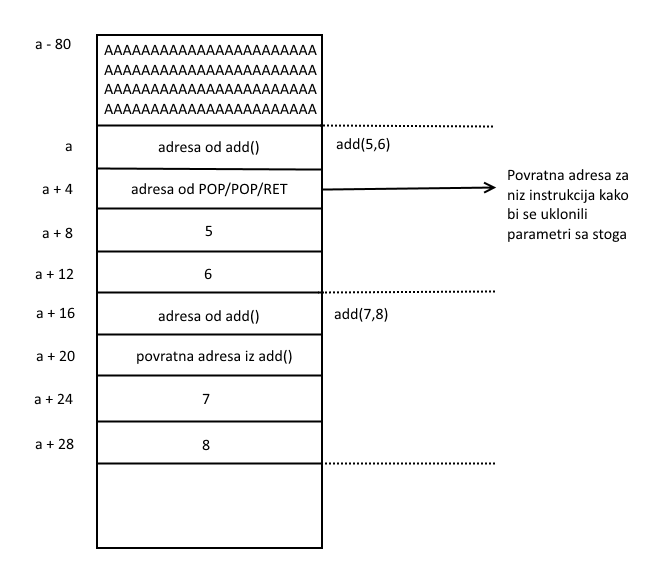
\includegraphics[width=12cm, height=12cm]{slike/rop_add78}
\caption{Izgled stoga nakon preljava u funkciji \emph{func1()}. Dvostruki poziv \emph{add()} funkciji.}
\label{fig:rop_add78} 
\end{figure}
Iz primjera prikazanih u ovom poglavlju vidljivo je kako programiranje temeljeno na "ret" blokovima predstavlja značajnu prijetnju za aplikacija koje su ranjive na napade tipa preljeva spremnika. Vjerojatno najveća opasnost koju programiranje temeljeno na "ret" blokovima predstavlja je potpuno zaobilaženje DEP mehanizma zaštite. Postavlja se stoga pitanje: Na koji način je moguće spriječiti ovaj oblik iskorištavanja propusta vezanih za korupciju memorije? 

Odgovor na to pitanje leži u randomizaciji dijelova programa i dijeljenih biblioteka koje program koristi. Upravo je tako i nastao mehanizam zaštite ASLR (\ref{sct:aslr}) koji značajno otežava napadaču pronalazak točnih lokacija određenih dijelova programskog koda koji bi se u konačnici mogli upotrijebiti prilikom konstruiranja potrebnih "ret" blokova. Međutim, ASLR ima nedostatke i moguće ga je zaobići. Ukoliko neki program koristi dijeljenu biblioteku kojoj nije omogućen ASLR (određuje se prilikom prevođenja), ta biblioteka će uvijek biti učitana na poznatu lokaciju te će napadač znati na kojim adresama se nalaze pojedini, zanimljivi dijelovi programskog koda koji se zatim mogu iskoristiti za konstrukciju "ret" blokova.

Uz ovaj rad napravljena je skripta u programskom jeziku Python(\emph{CheckAslrDep}) koja skenira sve PE datoteke u odabranom direktoriju te provjerava jesu li iste zaštićene ASLR i DEP sigurnosnim mehanizmima. Skripta je pokrenuta na potpuno ažuriranom operacijskom sustavu Microsoft Windows 7 Professional te je kao ciljani direktorij odabran \emph{C:\textbackslash Windows\textbackslash System32}. Navedeni direktorij odabran je iz razloga što se unutar njega nalaze sve važne sistemske DLL i EXE datoteke. Kao rezultat dobiveni su sljedeći podaci:
\begin{itemize}
\item Broj provjerenih PE datoteka: 3065
\item Broj datoteka sa ASLR zaštitom: 2583 (84\%)
\item Broj datoteka sa DEP zaštitom: 2575 (84\%)
\end{itemize}
Kao što je vidljivo iz priloženog, oko 500 sistemskih EXE i DLL datoteka nema ASLR ili DEP mehanizam zaštite aktivan. Napadač stoga lako može saznati o kojim se datotekama radi, te koje aplikacije koriste navedene datoteka. Na taj način, napadaču se pruža mogućnost da iskorištavanjem propusta u obliku preljeva spremnika u aplikaciji pristupi programskom kodu u nezaštičenim sistemskim datotekama te iskoristi isti za konstruiranje "ret" blokova.

Međutim, čak i ako je svim PE datotekama omogućen ASLR, moguće ga je zaobići. Jedan od načina je preko nesigurnih pokazivača (engl. \emph{Dangling/Leaking pointer}). U tom slučaju radi se o pokazivačima koji ne pokazuju na pravilan objekt u memoriju. Konkretno, oni mogu pokazivati na dio memorije koji je prethodno bio oslobođen. Upravo iz tog razloga, moguće je čitati navedene memorijske lokacije te dobiti uvid u način na koji se provodi randomizacija.


\chapter{PErmutator Program}
U prethodnim poglavljima obrađene su teme vezane za sam format PE
datoteka, za korupciju memorije te sigurnosne propuste koji istu
iskorištavaju. Također, obrađene su i teme vezane uz postojeće
mehanizme zaštite protiv napada usmjerenih na memoriju. Sve te
teme bilo je nužno proći kako bi se dobio dojam o tome koliko su
napadi usmjereni na memoriju još uvijek opasni te koliko su
određeni mehanizmi zaštite, koji se danas koriste, nedovoljno
sigurni kako bi se taj oblik napada u potpunosti iskorijenio.

U prethodnom poglavlju(\ref{sct:rop2}) pokazali smo i kako ASLR
kao randomizacijski mehanizam ima svojih nedostataka. Spomenuto
je i nekoliko tehnika preko kojih je moguće zaobići ASLR zaštitu
čak i kada ista postoji na sustavu. Glavni problem kod ASLR-a je
što se randomizacija provodi nad većim blokovima memorije. To
znači da se, primjerice početna adresa na koju se datoteka
učitava može mijenjati na slučajan način, ali sam sadržaj sekcije
koja sadrži programski kod će uvijek biti na istom odmaku od te
početne adrese. Glavni problem koji se tu javlja je sljedeći:
Ukoliko napadač uspije otkriti početnu adresu na koju je datoteka
učitana, on vrlo lako može doći do određenih vrijednosti u
sekciji sa programskim kodom jer su sve te vrijednosti uvijek na
istom odmaku. Navedeno je ilustrirano na slici
\ref{fig:aslr_permutacija}.

\begin{figure}[!htb]
\centering
\setlength\fboxsep{0pt}
\setlength\fboxrule{0.5pt}
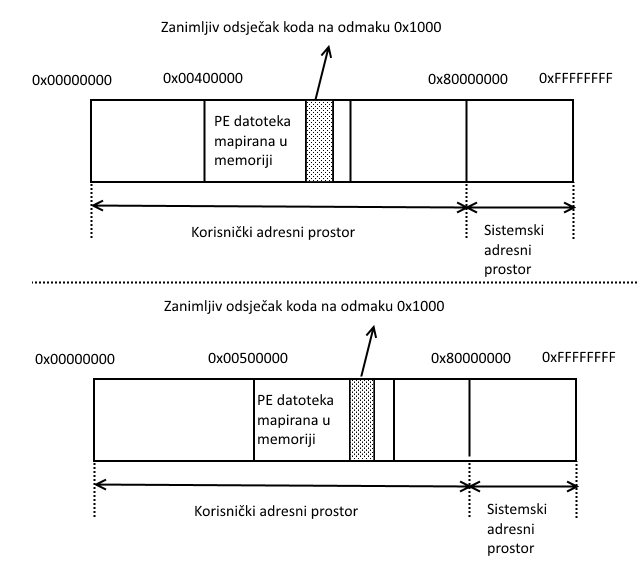
\includegraphics[width=12cm, height=12cm]{slike/aslr_permutacija}
\caption{Dijelovi koda su uvijek na istom odmaku od početne adrese na koju je PE datoteka učitana}
\label{fig:aslr_permutacija} 
\end{figure}

U ovakvim situacijama javlja se potreba za jednom novom,
detaljnijom vrstom randomizacije unutar procesnog adresnog
prostora. Konkretno, ideja iza modula za promjenu koda je
sljedeća: Uz randomizaciju koju nudi ASLR, potrebno je provesti
dodatnu permutaciju pojedinih dijelova sekcije koja sadrži
programski kod kako bi sam položaj tih dijelova prilikom svakog
pokretanja bio drugačiji. Na taj način zaštita bi se dodatno
poboljšala jer napadač više ne bi mogao iskoristiti činjenicu
kako se određeni interesni dijelovi programskog koda nalaze na
istom odmaku od početne adrese na koju je PE datoteka učitana u
memoriji. U konačnici, program bi imao potpuno drugačiji raspored
u memoriji pri čemu bi funkcionalnost ostala ista.

Razvoj jednog takvog modula za promjenu koda nije nimalo
jednostavan zadatak. Prije konstruiranja samog modula za promjenu
koda potrebno dati odgovore na nekoliko ključnih pitanja:

\begin{itemize}
\item Koje dijelove PE datoteka je potrebno permutirati i mijenjati?
\item Kako pronaći navedene dijelove unutar PE datoteke?
\item Na koji način su ti dijelovi međusobno povezani te kako utječu jedan na drugoga prilikom izvođenja programa?
\end{itemize}

Kako bi se moglo odgovoriti na prvo pitanje potrebno je dobro
poznavati format PE datoteka(poglavlje \ref{sct:peFormat}). Tu se
prije svega misli na sadržaj pojedinih sekcija, te što svaka od
njih sadrži. Pošto je razvoj jednog ovakvog modula namijenjen
poboljšanju sigurnosti uz postojeći ASLR mehanizam zaštite,
logičnim se čini kako bi promjena (permutacija) trebala zahvatiti
sekciju sa izvršnim kodom. Međutim, problem koji se tu javlja
proizlazi iz činjenice kako sekcija se izvršnim kodom često
sadrži i velike količine nepotrebnih okteta i dijelova koji se ne
izvrše niti u jednoj situaciji rada programa. 

Iz navedenoga proizlazi i sljedeće od ključnih pitanja: Kako
pronaći korisne, ključne dijelove sekcije s izvršnim kodom koji
bi trebali biti zahvaćeni permutacijom? Odgovor na to pitanje
leži u nekoj vrsti simulacije izvođenja programa. Konkretno,
počinje se od ideje kako prvi oktet koji će biti obuhvaćen
permutacijom je ujedno i prvi oktet prve instrukcije koja se
izvede. Navedeni položaj unutar sekcije s izvršnim kodom lako je
pronaći preko elementa \emph{AddressOfEntryPoint} koje je dio
opcionalnog zaglavlja unutar PE zaglavlja. U sljedećem koraku,
potrebno je odrediti sve moguće tokove programa počevši od
polazne točke (engl. \emph{Entry Point}) te na taj način
izgraditi graf instrukcija. Čvorovi u tom grafu su slijedne
instrukcije, tj. blokovi izvršnog koda koji bi se trebali
permutirati. Više o navedenome objašnjeno je u poglavlju
\label{sct:instrucionGraph}.

Posljednje pitanje na koje valja odgovoriti je ujedno i
najizazovnije. Razlog tome je što između pojedinih dijelova
programskog koda, koji se koriste u postupku permutacije, postoji
veliki broj referenci na ostale dijelove. Pronalazak navedenih
referenci i njihovo ažuriranje s obzirom na novi raspored u
memoriji je izuzetno zahtjevan zadatak. Mnoge od tih referenci je
nemoguće odrediti u postupku statičke analize. Osim toga navedeni
modul trebao bi biti konstruiran na način da ne uzrokuje značajan
pad performansi. Više o navedenom problema moguće je pročitati u
poglavlju \ref{sct:permutator}.

Kako bi modul za permutaciju koda bilo što jednostavnije
konstruirati, predloženi su sljedeći ključni dijelovi od kojih bi
se modul trebao sastojati:

\begin{itemize}
\item Disasembler dio
\item Funkcije za rad s PE datotekama
\item Dio za konstrukciju grafa instrukcija
\item Permutator dio
\end{itemize}

U nastavku ovog poglavlja svaki od pojedinih dijelova je detaljno
analiziran. Opisan je način na koji je pojedini dio implementiran
te koja je njegova funkcija u konačnom proizvodu. Valja još
napomenuti kako je cijeli projekt moguće pratiti na stranici
Github: https://github.com/bhumic/PErmutator

\pagebreak

\section{Disasembler}

Disasembler je ključan dio za provedbu bilo kakve manipulacije
nad izvršnim kodom kod PE datoteka. U prethodnom poglavlju
spomenuta je izgradnja grafa instrukcija. Kako bi se u gradnju
grafa instrukcija uopće moglo krenuti, potrebno je unaprijed
definirati sadržaj pojedinih čvorova u grafu te način na koji su
isti povezani. Pošto znamo kako će sadržaj pojedinih čvorova biti
izvršni programski kod, tj. svaki čvor će sadržavati određenu
količinu slijednih instrukcija procesora, nužno je stvoriti
mehanizma pomoću kojega će se te instrukcije dobiti iz sirovih
podataka (okteta). To je potrebno iz razloga što je jednostavnije
upravljati nizovima okteta ukoliko te iste nizove imamo u
smislenim tekstualnim reprezentacijama.

Gradnja jednoga takvog alata kao što je disasembler nije nimalo
jednostavan zadatak. Na današnjim, modernim x86 procesorima
postoje stotine mogućih instrukcija te konstrukcija disasemblera
od početka je posao koji bi zahtijevao jako mnogo vremena. Na
sreću, danas postoje mnoge gotove biblioteke koje nude
funkcionalnost disasemblera za velik broj programskih jezika.
Pošto sam ja ovaj rad odlučio raditi u C++ programskom jeziku,
logičnim se pokazalo pronaći odgovarajuću biblioteku koja nudi
funkcionalnost disasemblera.

Možda će nekome biti iznenađujuće, ali ne postoji velik broj
kvalitetnih disasembler biblioteka za programski jezik C++. U
konačnici izbor se sveo na dvije biblioteka:
\emph{Distorm}\citep{distorm} i
\emph{BeaEngine}\citep{bea_engine} pri čemu je pobjedu uzeo
\emph{Distorm}.

\emph{Distorm} je izuzetno moćna i brza disasembler biblioteka
koja nudi podršku za dosta programskih jezika osim C/C++. Moguće
je biblioteku koristiti i za projekte u Pythonu, Javi te C\#-u.
Također, osim jednostavne pretvorbe sirovih okteta u smisleni
tekstualni zapis, \emph{Distorm} cijeli disasemblerski postupak
provodi na način što konstruira strukturu u programskom jeziku
C++ preko koje je moguće pristupati određenim, ciljanim
dijelovima dekodirane instrukcije. Sadržaj strukture prikazan je
na odsječku koda \ref{lst:distorm} te se na taj način postupak
analize binarnih x86 datoteka dodatno pospješuje. Više o samoj
\emph{Distorm} biblioteci moguće je pročitati na službenim
stranicama projekta\citep{distorm}. 

\pagebreak
\begin{lstlisting}[frame=single, caption=Temeljna \emph{distorm} struktura za dekodiranu instrukciju, label={lst:distorm}]
typedef struct {
	_WString mnemonic; /* Tekstualni naziv instrukcije. */
	_WString operands; /* Operandi dekodirane instrukcije. */
	_WString instructionHex; /* Heksadecimalni zapis instrukcije */
	unsigned int size; /* Velicina dekodirane instrukcije u oktetima */
	_OffsetType offset; /* Pomak na kojemu se instrukcija nalazi */
} _DecodedInst;
\end{lstlisting}

\section{Funkcije za Rad s PE Datotekama}

U prošlom poglavlju rečeno je kako je za rad s izvršnim kodom PE
datoteka nužno postojanje alata kao što je disasembler. Međutim,
prije nego se nakupina okteta koja čini izvršni kod provede kroz
disasembler, nužno je na neki način odvojiti te oktete od ostatka
datoteke. Također, prilikom permutacije dijelova izvršnog koda
nužno je napraviti i promjene u određenim zaglavljima PE
datoteka. Neke od promjena su modifikacija početne točke (engl.
\emph{Entry Point}) programa ili promjene u zaglavlju sekcije
ukoliko dolazi do promjene u veličini sekcije ili karakteristike
sekcije. Iz navedenih razloga bilo je potrebno uvesti skupinu
funkcija pomoću kojih se sve operacije, vezane za manipulaciju
sadržajem PE datoteka, značajno pojednostavljuju. U nastavku
slijedi popis i opis funkcija za rad s PE datotekama koje su
implementirane za potrebe ovog rada. Navedene funkcije moguće je
koristiti i za razvoj drugih alata koji na neki način obavljaju
analiza sadržaja PE datoteka. Radi preglednog ispisa sve funkcije
navedene su bez argumenata koje primaju. Za detaljniju analizu
pojedinih funkcija preporučam uvid u datoteke
\emph{PEFunctions.h} i \emph{PEFunctions.cpp} koje su priložene
ovom radu. Popis funkcija:

\begin{itemize}

\item {\footnotesize \emph{BYTE* LoadSection((std::fstream\&
hFile, PIMAGE\_SECTION\_HEADER pSectionHeader))}}: Navedena
funkcija prima referencu na otvorenu PE datoteku te pokazivač na
strukturu koja opisuje zaglavlje sekcije. Iz navedenih ulaznih
parametara, funkcija čita te vraća sadržaj odabrane sekcije.

\item {\footnotesize \emph{BOOL WriteSection(std::ofstream\&
hFile, PIMAGE\_SECTION\_HEADER pSectionHeader, unsigned char
*buffer)}}: Funkcija koja zapisuje novi sadržaj odabrane sekcije
u PE datoteku.

\item {\footnotesize \emph{LPVOID ReadHeader(std::fstream\&
hFile, DWORD dwHeaderSize, DWORD dwOffset)}}: Funkcija koja, na
temelju veličine zaglavlja i odmaka zaglavlja od početka
datoteke, učitava zaglavlje u memoriju kako bi isto mogli biti
spremno za daljnju manipulaciju.

\item {\footnotesize \emph{PIMAGE\_SECTION\_HEADER
FindSection(std::fstream\& hFile, DWORD dwRVA, DWORD
dwFstSectionHeader, WORD wNumSections)}}: Funkcija koja s obzirom
na relativnu virtualnu adresu vraća pokazivač na strukturu
sekcije unutar koje se navedena adresa nalazi.

\item {\footnotesize \emph{DWORD AlignUp(DWORD dwSize, DWORD
dwAlign)}}: Funkcija koja željenu vrijednost zaokružuje na
višekratnik argumenta \emph{dwAlign}.

\item {\footnotesize \emph{BYTE* ReadData(unsigned char*buffer,
DWORD dwOffset, DWORD dwSize)}}: Funkcija koja s obzirom na
posmak od početka datoteke te s obzirom na veličinu, čita željeni
broj okteta iz datoteke.

\item {\footnotesize \emph{BOOL
WriteSectionHeader(PIMAGE\_SECTION\_HEADER pSectionHeader, DWORD
dwSectionID, std::ofstream\& hFile, DWORD
dwFstSctHeaderOffset)}}: Funkcija koja odabrano zaglavlje sekcije
zapisuje na odgovarajuće mjesto unutar PE datoteke.

\item {\footnotesize \emph{PIMAGE\_SECTION\_HEADER
AddSection(std::fstream\& hFile, unsigned char *sectionData,
DWORD dwSectionDataSize, DWORD dwFstSectionHeaderOffset,
PIMAGE\_NT\_HEADERS pNtHeader, const char *sectionName)}}:
Funkcija koja dodaje novu sekciju (uključujući i zaglavlje
sekcije) na određeno mjesto unutar PE datoteke.

\item {\footnotesize \emph{BYTE*
LoadExecutableSection(std::fstream\& hFile, PIMAGE\_DOS\_HEADER
pDosHeader, PIMAGE\_NT\_HEADERS pNtHeader, DWORD
dwFstSctHdrOffset, PIMAGE\_SECTION\_HEADER* pSectionHeader)}}:
Funkcija koja u memoriju učitava sadržaj sekcije sa izvršnim
kodom.

\item {\footnotesize \emph{BOOL ValidateFile(std::fstream\&
hFile)}}: Funkcija koja provjerava je li odabrana PE datoteka
valjana.

\end{itemize}

\section{Graf Instrukcija}
\label{scr:instructionGraph}
Konstruiranje grafa instrukcija jedan je od najvažnijih zadataka vezanih za implementaciju programa poput modula za promjenu koda. U ovom poglavlju opisan je način na koji je jedan takav graf konstruiran. Preciznije, u nastavku poglavlja slijedi detaljan opis pojedinih elemenata grafa te samog algoritma konstrukcije grafa. Osim opisa samog grafa i njegove primjene unutar modula za promjenu koda, ovo poglavlje sadrži i ostale načine na koje je navedeni graf moguće primijeniti. 

Dobro je poznato kako se svaki graf sastoji od dvaju osnovnih skupova: skup čvorova i skup bridova. Iz tog razloga, prije nego krenemo u opis implementacije grafa, potrebno je definirati što je u našem grafu obuhvaćeno čvorovima, a što bridovima. Pošto se unutar ovog projekta konstruira graf instrukcija, logično je za pretpostaviti kako će čvorovi unutar grafa biti slijedne grupe instrukcija, dok će bridovi prikazivati određene veze među tim grupama instrukcija. Postoji nekoliko načina na koje se može definirati veza između pojedinih vrhova. Međutim, s obzirom na karakteristiku grafa koji gradimo, odlučeno je kako će veza između pojedinih vrhova ovisiti o položaju instrukcija skoka unutar programskog koda. Na taj način, graf koji se gradi u ovom projektu je zapravo graf toka izvođenja (engl. \emph{Control Flow Graph}). Kako bi bilo jasnije, prikaz jednog takvog grafa nalazi se na slici \ref{fig:control_flow_graph}.

\begin{figure}[!htb]
\centering
\setlength\fboxsep{0pt}
\setlength\fboxrule{0.5pt}
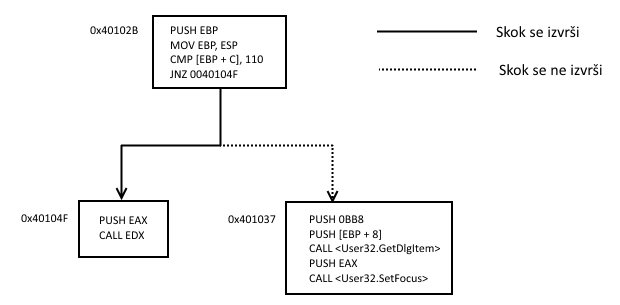
\includegraphics[width=13cm, height=8cm]{slike/control_flow_graph}
\caption{Primjer grafa toka izvođenja.}
\label{fig:control_flow_graph} 
\end{figure}
Kao što je vidljivo na slici \ref{fig:control_flow_graph}, dva su čvora povezana ukoliko postoji mogućnost da program prilikom izvršavanja instrukcija u jednome čvoru počne izvršavati instrukcije u drugome čvoru. To znači da svaki čvor, kojemu je posljednja instrukcija uvjetni skok, ima vezu prema dva čvora. Jedan od ta dva čvora sadrži instrukcije koje će se izvršiti ukoliko je uvjet za skok istinit, dok drugi sadrži instrukcije koje će se izvršiti kada je uvjet za skok neistinit, tj. kada do skoka ne dođe. Osim uvjetnog skoka, moguće je da posljednja instrukcija unutar čvora bude instrukcija bezuvjetnog skoka. U tom slučaju postoji samo jedna veza jer ne postoji nikakvo ispitivanje uvjeta skoka, tj. skok se uvijek događa.

Prije nego krenemo u sam opis algoritma za konstrukciju grafa instrukcija te njegovu pohranu u memoriji za daljnju obradu, potrebno je opisati na koji način su implementirani vrhovi i bridovi unutar ovog projekta. Vrhovi su definirani unutar datoteke \emph{Node.h} čiji najvažniji dijelovi se nalaze na odsječku koda \ref{lst:node}. 

\begin{lstlisting}[frame=single, caption=Klasa koja opisuje vrh(čvor) grafa instrukcija, label={lst:node}]
class Node
{
public:
	Node();
	~Node();

	int AppendChild(Node* child);
	Node* FindChild(DWORD offset);

	bool operator==(const Node& node);
private:
	DWORD dwOffset;
	DWORD dwSize;
	BYTE* instructions;
	std::vector<Node* > children;
};
\end{lstlisting}
Postoji nekoliko ključnih funkcija i varijabli unutar klase koja opisuje vrhove stoga su oni opisani u nastavku:
\begin{itemize}
\item \emph{AppendChild(Node* child)}: Funkcija koja trenutnom čvoru dodaje dijete čvor. Preciznije, ovom funkcijom stvara se veza između trenutnog čvora i čvora \emph{child}. To znači da su navedena dva čvora povezana preko uvjetnog ili bezuvjetnog skoka. Također, valja napomenuti kako je ova metoda konstruirana na način da sprječava postojanje petlji, tj. ukoliko se pokuša kao dijete dodati čvor prema kojemu veza već postoji, isti neće biti dodan te će funkcija vratiti pravilnu povratnu vrijednost.
\item \emph{FindChild(DWORD)offset}: Funkcija koja vraća pokazivač na čvor dijete kojemu odgovara argument \emph{offset}.
\item \emph{dwOffset}: Navedena vrijednost je jedinstveni ključ za svaki čvor(vrh). Označava gdje se promatrani čvor nalazi s obzirom na početak sekcije sa izvršnim kodom.
\item \emph{dwSize}: Označava veličinu čvora, tj. broj okteta unutar čvora.
\item \emph{instructions}: Sadrži \emph{dwSize} broj okteta koji označavaju instrukcije koje se nalaze unutar navedenog čvora. Ovaj element sadrži sam sadržaj čvora.
\item \emph{children}: Vektor koji sadrži svu djecu trenutnog čvora. Navedeni vektor može imati najviše dva elementa ili najmanje nula elemenata. Ukoliko vektor sadrži dva elementa, zna se da je posljednja instrukcija unutar čvora instrukcija uvjetnog skoka. Ako vektor sadrži nula elemenata tada se radi o posljednjem čvoru u grafu, tj. u čvoru iz kojeg nema daljnjeg izvršavanja. Ovim elementom su zapravo opisani i bridovi (veze) unutar grafa.
\end{itemize}
Sada kada smo opisali osnovne elemente grafa instrukcija možemo krenuti sa detaljnim opisom algoritma za njegovu konstrukciju. U prva dva poglavlja ove cjeline bilo je govora o disasembleru i funkcijama za rad s PE datotekama. Oba ta dijela su od velike važnosti za sam postupak konstruiranja grafa instrukcija.

Funkcije za rad s PE datotekama su potrebne kako bi se izdvojila sekcija sa izvršnim kodom. Upravo su dijelovi te sekcije sačuvani unutar pojedinih čvorova unutar grafa te se sam postupak izgradnje provodi prolaskom kroz sadržaj te sekcije. Disasembler je važan dio u postupku konstrukcije grafa jer nam na jednostavan način pomaže pronaći instrukcije skoka.

Programski kod, koji obavlja operaciju konstrukcije grafa instrukcija te njegovu pohranu u memoriji, opisan je u datoteci \emph{Permutator.cpp} unutar funkcija \emph{CreateGraph()} i \emph{\_CreateGraph()}. Što se tiče samog algoritma, radi se o rekurzivnom algoritmu koji je detaljno opisan u nastavku:
\begin{enumerate}
\item Potrebno je izračunati na kojem odmaku od početka sekcije s izvršnim kodom se nalazi početna točka izvršavanja (engl. \emph{Entry Point}). Navedena operacija događa se unutar funkcije \emph{CreateGraph()}. Nakon što se odmak odredi poziva se rekurzivna funkcija \emph{\_CreateGraph()}. Njeni parametri opisani su u nastavku:
\begin{itemize}
\item \emph{BYTE* sectionData}: Pokazivač na sadržaj sekcije s izvršnim kodom
\item \emph{\_OffsetType blockOffset}: Odmak od početka sekcije. Označava od koje pozicije unutar sekcije s izvršnim kodom počinje blok instrukcija koji je sadržan unutar pojedinog čvora grafa.
\item \emph{DWORD dwSectionSize}: Veličina sekcije s izvršnim kodom. Ova vrijednost se mijenja prilikom rekurzivnog pozivanja. Ovisi o vrijednosti \emph{blockOffset}, tj. označava broj okteta između pomaka definiranog sa \emph{blockOffset} i kraja sekcije.
\item \emph{\_OffsetType parentOffset}: Označava na kojoj poziciji unutar sekcije s izvršnim kodom se nalazi čvor koji predstavlja roditelja trenutnom čvoru.
\end{itemize} 
\item Potrebno je sadržaj sekcije provesti kroz disasembler, počevši od početne točke izvršavanja (engl. \emph{Entry Point.}).
\item U ovome koraku dobiven je tekstualni prikaz instrukcija iz disasemblera te se ovaj korak sastoji od dvaju manjih koraka. Prvu stvar koju je potrebno napraviti je provjeriti redom instrukcije sve dok ne dođemo do instrukcija \emph{RET}, \emph{RETN}, \emph{DB} ili neke od instrukcija skoka.
\begin{enumerate}
\item Ukoliko je pročitana instrukcija \emph{RET}, \emph{RETN} ili \emph{DB} potrebno je zabilježiti njen položaj s obzirom na početak sekcije. U tom trenutku potrebno je izgraditi novi čvor koji će sačinjavati instrukcije od početka bloka (\emph{blockOffset}) do pojave instrukcije \emph{RET}, \emph{RETN} ili \emph{DB}. Taj novi čvor se zatim dodaje u graf te se obavlja povratak iz funkcije \emph{\_CreateGraph()} na višu razinu rekurzije.
\item Ukoliko je pročitana instrukcija uvjetnog ili bezuvjetnog skoka potrebno je, kao i u prethodnom koraku, zabilježiti položaj iste te izgraditi novi čvor. Međutim, za razliku od prethodnog koraka gdje se instrukcije \emph{RET} i \emph{RETN} tretiraju kao završni dijelovi rekurzije, instrukcije skoka osiguravaju još barem jedan poziv funkcije \emph{\_CreateGraph()}. Razlog tome je što ako trenutni čvor završava instrukcijom uvjetnog skoka, taj čvor će imati sigurno dvije veze, tj. dva čvora djeteta. Svaki uvjetni skok uzrokuje dva moguća smjera u kojima izvođenje programa može krenuti te je upravo to razlog zašto treba nastaviti s rekurzivnima pozivima prema \emph{\_CreateGraph()} funkciji.
\end{enumerate}
\end{enumerate} 
Ovime dolazimo do kraja poglavlja o grafu instrukcija. Za kraj valja još napomenuti nekoliko stvari. U ovome konkretnom primjeru, kao veze između čvorova korištene su instrukcije skoka. Međutim, ranije unutar poglavlja spomenuto je kako veze između čvorova mogu biti definirane na razne načine. Jedan od dodatnih načina je i korištenje poziva funkcija. Na taj način moguće je izdvojiti funkcije kao zasebne čvorove te provoditi određene operacije nad njima. Primjer grafa i pripadajućih mu instrukcija generiranog pomoću razvijenog modula moguće je vidjeti u dodatku \ref{sct:appPE} i dodatku \ref{sct:appGraph}.

Za sam kraj valja još spomenuti nekoliko područja gdje se graf instrukcija može primijeniti. Osim za gradnju modula za promjenu koda, graf instrukcija moguće je primijeniti prilikom konstruiranja nekih složenijih disasemblera kako bi se dobio pregledniji prikaz toka programa. Jedan od primjera takve primjene je i poznati disasembler alat \emph{Ida Pro}\citep{ida}. Postojanje grafa instrukcija u memoriji može se, osim za pregledniji prikaz, iskoristiti i prilikom konstruiranja alata čija zadaća je zaštiti programski kod od postupaka reverznog inženjeringa. Za primjer, moguće je kriptirati pojedine čvorove grafa različitim tehnikama te uvesti određene anti-debug tehnike između pojedinih čvorova. U sljedećem poglavlju opisana je ideja permutacije pojedinih čvorova grafa te problemi koji su se u tom postupku pojavili.

\section{Permutator}
\label{sct:permutator}
Ovo poglavlje sadrži opis ideje o postupku permutacije čvorova grafa instrukcija. Detaljno je opisana ideja o načinu permutacije te su navedeni problemi s kojima smo se susreli i koji su, nažalost, onemogućili da se ovaj projekt razvije do kraja unutar roka.

Kao što smo naveli u prethodnom poglavlju, svaki čvor unutar grafa instrukcija ima jedinstveni identifikator. Taj identifikator je zapravo odmak od početka sekcije s izvršnim kodom te je opisan preko elementa \emph{blockOffset}. Ideja kod permutacije grafa instrukcija je sljedeća: Uzmimo dva čvora. Neka se prvi nalazi na odmaku \emph{a}, dok se drugi nalazi na odmaku \emph{b}. Potrebno je navedena čvorove zamijeniti tako da se sada prvi nalazi na odmaku \emph{b} te da se drugi nalazi na odmaku \emph{a}. Iako se čini kao dosta jednostavna ideja, njezina implementacija je krajnje komplicirana te se susrećemo sa problemima.

Najveći problem kod konstruiranja jednoga ovakvog alata su reference, tj. ažuriranje svih referenci u svim čvorovima koji su na neki način ovisni o čvoru koji mijenja svoju poziciju (odmak od početka sekcije). U početku se čini kako bi se navedeni problem mogao riješiti razvojem efikasnog algoritma i skupa tablica preko kojih bi se veze između pojedinih čvorova pratile. Međutim, u stvarnosti je to malo drugačije. U ranijim poglavljima spomenuto je kako se kod programiranja u asembleru argumenti funkcijama prenose putem stoga. Prilikom statičke analize PE datoteke, nemoguće je odrediti koje od tih argumenata je potrebno ažurirati prilikom mijenjanja lokacije čvora. Razlog tome je što neki od tih argumenata označavaju konstante koje nikako ne bi trebalo mijenjati, dok drugi dijelovi označavaju adrese koje bi trebalo promijeniti. Glavni problem koji se ovdje nameće je kako razlikovati konstante od adresa. 

Postoji nekoliko opcija kako bi se navedeno moglo riješiti. Jedna opcija je korištenjem tablice relokacija. Tablica relokacija sadrži popis svih mjesta unutar PE datoteke gdje je potrebno obaviti relokaciju ukoliko datoteka nije učitana na željenu početnu adresu. U tom slučaju su sve apsolutne adrese unutar programskog koda nepravilne te ih je potrebno promijeniti (relocirati). Međutim, prvi problem s relokacijama je što ne sadrže sve PE datoteke sekciju sa relokacijskom tablicom. Takve datoteke, ukoliko se pojavi potreba za relokacijom, neće raditi pravilno. Druga opcija je imati popis funkcija iz Windows API-a te na osnovu import tablice odrediti koja funkcija se poziva. Na taj način moguće je točno znati koji argument je adresa a koji argument je konstanta. Međutim, veliki problem kod ovog rješenja je što postoje tisuće funkcija iz Windows API-a. Neke od tih funkcija su dokumentirane, dok neke nisu. Pretraživati jednu tako veliku bazu bez zajamčenog uspjeha zahtjeva veliku računalnu moć, te se time jedan alat poput modula za promjenu koda ne bi isplatio. Kako bi sve prethodno navedeno bilo jasnije potrebno je pogledati sljedeći primjer. Na odsječku koda \ref{lst:PE_instructions} nalazi se dio instrukcija iz jedne jednostavne PE datoteke (odsječak instrukcija počinje na adresi \emph{0x00401000}).

\begin{lstlisting}[frame=single, caption=Instrukcije unutar PE datoteke, label={lst:PE_instructions}]
6A 00	                      PUSH 0
E8 45010000                   CALL <JMP.&KERNEL32.GetModuleHandleA>
A3 54304000                   MOV DWORD PTR DS:[403054],EAX
6A 00                         PUSH 0                           
68 2B104000                   PUSH AD_CM#1.0040102B                    
6A 00                         PUSH 0                                    
68 00304000                   PUSH AD_CM#1.00403000                        
FF35 54304000                 PUSH DWORD PTR DS:[403054]                   
E8 F7000000                   CALL <JMP.&USER32.DialogBoxParamA>           
50                            PUSH EAX                                    
E8 1B010000                   CALL <JMP.&KERNEL32.ExitProcess>         
55                            PUSH EBP
8BEC                          MOV EBP,ESP
817D 0C 10010000              CMP DWORD PTR SS:[EBP+C],110
75 18                         JNZ SHORT AD_CM#1.0040104F
68 B80B0000                   PUSH 0BB8                                 
FF75 08                       PUSH DWORD PTR SS:[EBP+8]               
E8 E4000000                   CALL <JMP.&USER32.GetDlgItem>                 
50                            PUSH EAX                                       
E8 F6000000                   CALL <JMP.&USER32.SetFocus>                    
E9 C4000000                   JMP AD_CM#1.00401113
\end{lstlisting}
Kao što je vidljivo na odsječku koda, postoje dvije instrukcije skoka. Prva instrukcija skoka je instrukcija uvjetnog skoka koja se nalazi u 15. redu, dok je druga instrukcija bezuvjetnog skoka i nalazi se u posljednjem, 21. redu odsječka koda \ref{lst:PE_instructions}. Također, valja obratiti pozornost na 5. redak gdje se vrijednost \emph{0x0040102B} postavlja na stog. Navedena vrijednost označava pokazivač na funkciju koja se izvršava prilikom poziva Windows API funkcije \emph{DialogBoxParamA} u retku 8. Graf instrukcija koji je moguće generirati iz navedenog odsječka koda prikazan je na slici \ref{fig:control_flow_graph_pe}.

\begin{figure}[!htb]
\centering
\setlength\fboxsep{0pt}
\setlength\fboxrule{0.5pt}
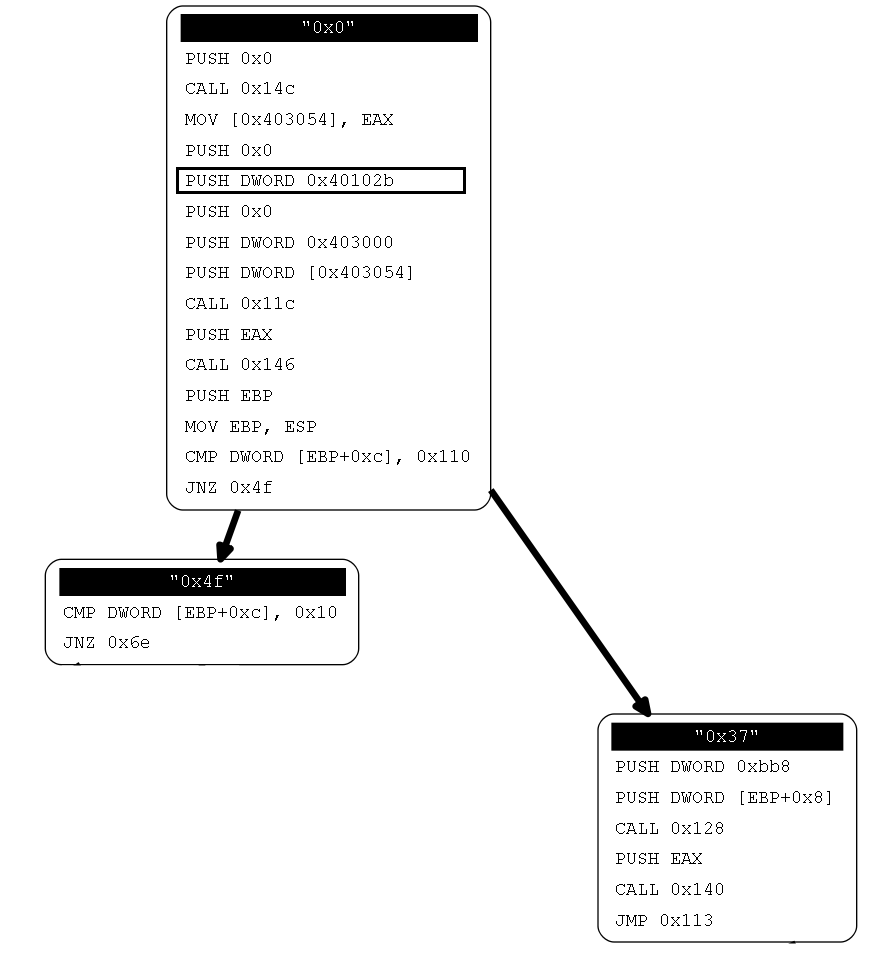
\includegraphics[width=10cm, height=8cm]{slike/permutator_graph_part}
\caption{Graf instrukcija za odsječak koda \ref{lst:PE_instructions}.}
\label{fig:control_flow_graph_pe} 
\end{figure}
Zamislimo sada sljedeći scenarij: Neka se dani odsječak koda preda kao ulazni podatak u modul za permutaciju te neka se permutacija odvija na način da se blok na odsječku \emph{0x0} zamijeni sa blokom na odsječku \emph{0x37} (radi se o dvama susjednim blokovima, tj. koji slijede jedan iza drugoga u memoriji). Problem koji se ovdje javlja upravo je vezan za postavljanje vrijednosti \emph{0x0040102B} na stog. Navedena adresa pokazuje na 12. redak u odsječku koda \ref{lst:PE_instructions}. Nakon što se permutacija provede, navedena adresa više neće biti valjana jer se cijeli blok pomakao za određenu vrijednost, tj. za vrijednost veličine bloka na odsječku \emph{0x37}. Kako bi nova datoteka bila ispravna, potrebno je, između ostaloga, ispraviti vrijednost \emph{0x0040102B}. Međutim, glavni problem ovdje je kako znati da se \emph{0x00401002B} odnosi na adresu, a ne, primjerice, na konstantu. U ovome slučaju je to lako odrediti jer imamo poziv prema \emph{DialogBoxParam} funkciji, ali vrlo lako se moglo dogoditi da je umjesto poziva prema Windows API funkciji bio poziv oblika \emph{CALL EAX} pri čemu bi vrijednost \emph{0x0040102B}, koja se postavlja na stog, imala potpuno drugo značenje. Pripadni graf instrukcija, nakon provedene permutacije, prikazan je na slici \ref{fig:control_flow_graph_permutated}. Ovdje valja obratiti pažnju na uokvirene vrijednosti na slici \ref{fig:control_flow_graph_pe} i \ref{fig:control_flow_graph_permutated}.

\begin{figure}[!htb]
\centering
\setlength\fboxsep{0pt}
\setlength\fboxrule{0.5pt}
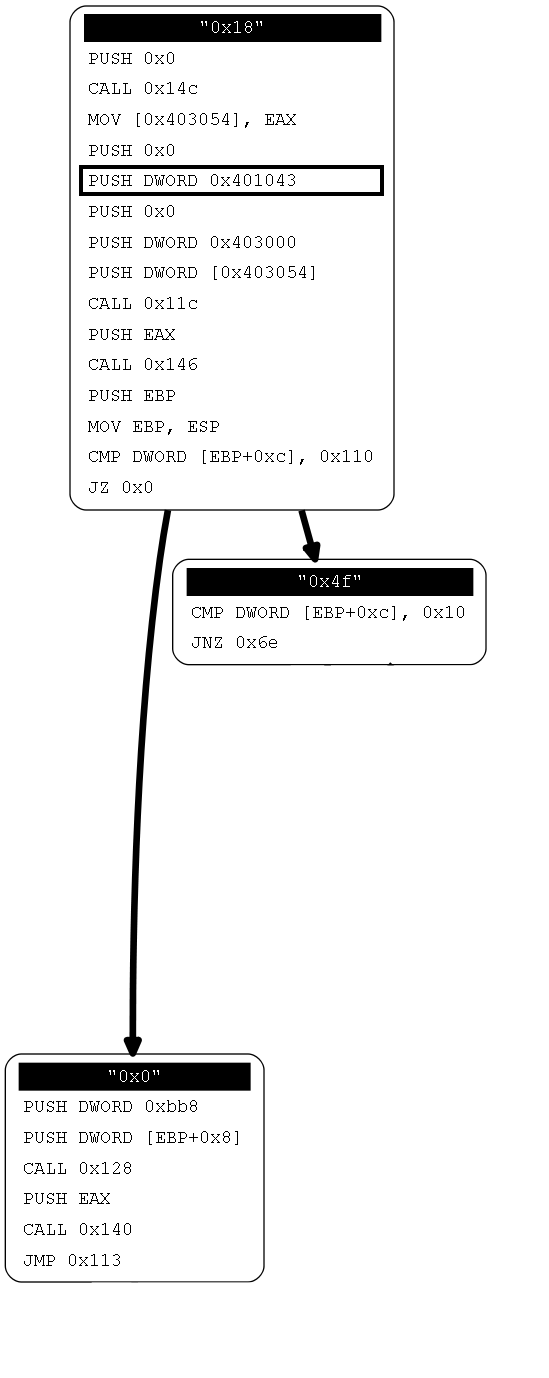
\includegraphics[width=8cm, height=14cm]{slike/permutator_graph_permutated}
\caption{Graf instrukcija za odsječak koda \ref{lst:PE_instructions} nakon provedene permutacije.}
\label{fig:control_flow_graph_permutated} 
\end{figure}
Prije nego završimo s ovim poglavljem, valja spomenuti još jedno moguće rješenje za problem oko ažuriranja referenci. Radi se o heurističnom rješenju te ga je najbolje objasniti korištenjem prethodnog primjera.

Kao što je prethodno navedeno, glavni problem sa permutacijom odsječka koda \ref{lst:PE_instructions} je postavljanje vrijednosti \emph{0x00401002B} na stog jer ne možemo sa sigurnošću reći radi li se o adresi ili o konstanti. Međutim, možemo krenuti od pretpostavke da ukoliko vrijednost koja se postavlja na stog pripada negdje unutar sekcije sa izvršnim kodom, tada ta vrijednosti označava adresu a ne konstantu. U gornjem slučaju takva pretpostavka bi nas dovela do pravilne permutacije i nove PE datoteke koja radi bez pogreške. Nažalost, navedena funkcionalnost još nije u potpunosti implementirana te se radi na tome.


\chapter{Zaključak}
U ovome radu bavili smo se novim tehnikama randomizacije
memorijskog rasporeda kod PE datoteka karakterističnih za
Microsoft Windows operacijski sustav. Svrha rada bila je
istražiti te poboljšati sigurnost operacijskog sustava na napade
koji iskorištavaju korupciju memorije. Tu se prije svega misli na
napade poput programiranja zasnovanog na "ret" blokovima, koje je
danas najučestaliji oblik iskorištavanja memorijskih ranjivosti.

U sklopu rada započet je razvoj alata koji bi omogućio potpuno
drugačiji raspored memorijskih blokova unutar sekcije sa izvršnim
kodom, pritom zadržavajući svu funkcionalnost originalne PE
datoteke. Time bi se otpornost na određene metode napada na
memoriju značajno poboljšala. Iako alat nije do kraja razvijen, u
radu je moguće pročitati sve o problemima s kojima smo se tijekom
implementacija susreli te moguća rješenja kako te probleme
riješiti. Osim samog alata za permutaciju, u radu se nalazi
detaljan opis postojećih sigurnosnih mehanizama koji su zasnovani
na randomizaciji te je dan detaljan opis najučestalijih napada
vezanih za korupciju memorije.

Nadam se da će se rad na jednom ovakvom alatu nastaviti u
budućnosti jer pruža jedan sasvim novi uvid u metode zaštite.
Dobro je poznato kako svi napadi usmjereni na korupciju memorije
iskorištavaju pogreške programera. Takvih pogrešaka će uvijek
biti jer ljudi jednostavno nisu savršeni i griješe tokom rada,
stoga je glavna prednost ovog i sličnih alata što umjesto da
popravljaju postojeće sigurnosne propuste, oni značajno otežavaju
napadačima pronalaženje takvih propusta te samim time i njihovo
iskorištavanje.

\bibliography{literatura}
\nocite{*}
\bibliographystyle{fer}

\appendix

\chapter{Primjer instrukcija iz PE datoteke}
\label{sct:appPE}

U nastavku ovog dodatka nalazi se odsječak koda
\ref{lst:PE_instructions_full} iz jedne PE datoteke. Radi se o
svim instrukcijama iz sekcije sa izvršnim kodom. Postojanje ovih
instrukcija nužno je za razumijevanje grafa instrukcija koji se
nalazi u dodatku \ref{sct:appGraph}.

\begin{lstlisting}[frame=single, caption=Instrukcije unutar PE datoteke, label={lst:PE_instructions_full}]
6A 00	                      PUSH 0
E8 45010000                   CALL <JMP.&KERNEL32.GetModuleHandleA>
A3 54304000                   MOV DWORD PTR DS:[403054],EAX
6A 00                         PUSH 0                           
68 2B104000                   PUSH AD_CM#1.0040102B                    
6A 00                         PUSH 0                                    
68 00304000                   PUSH AD_CM#1.00403000                        
FF35 54304000                 PUSH DWORD PTR DS:[403054]                   
E8 F7000000                   CALL <JMP.&USER32.DialogBoxParamA>           
50                            PUSH EAX                                    
E8 1B010000                   CALL <JMP.&KERNEL32.ExitProcess>         
55                            PUSH EBP
8BEC                          MOV EBP,ESP
817D 0C 10010000              CMP DWORD PTR SS:[EBP+C],110
75 18                         JNZ SHORT AD_CM#1.0040104F
68 B80B0000                   PUSH 0BB8                                 
FF75 08                       PUSH DWORD PTR SS:[EBP+8]               
E8 E4000000                   CALL <JMP.&USER32.GetDlgItem>                 
50                            PUSH EAX                                       
E8 F6000000                   CALL <JMP.&USER32.SetFocus>                    
E9 C4000000                   JMP AD_CM#1.00401113
837D 0C 10                    CMP DWORD PTR SS:[EBP+C],10
75 19                         JNZ SHORT AD_CM#1.0040106E
6A 00                         PUSH 0              
68 027D0000                   PUSH 7D02 
68 11010000                   PUSH 111 
FF75 08                       PUSH DWORD PTR SS:[EBP+8] 
E8 D1000000                   CALL <JMP.&USER32.SendMessageA> 
E9 A5000000                   JMP AD_CM#1.00401113
817D 0C 11010000              CMP DWORD PTR SS:[EBP+C],111
0F85 8F000000                 JNZ AD_CM#1.0040110A
8B45 10                       MOV EAX,DWORD PTR SS:[EBP+10]
837D 14 00                    CMP DWORD PTR SS:[EBP+14],0
75 16                         JNZ SHORT AD_CM#1.0040109A
66:3D 027D                    CMP AX,7D02
0F85 85000000                 JNZ AD_CM#1.00401113
6A 00                         PUSH 0 
FF75 08                       PUSH DWORD PTR SS:[EBP+8]
E8 8A000000                   CALL <JMP.&USER32.EndDialog>
EB 79                         JMP SHORT AD_CM#1.00401113
8B55 10                       MOV EDX,DWORD PTR SS:[EBP+10]
C1EA 10                       SHR EDX,10
66:0BD2                       OR DX,DX
75 63                         JNZ SHORT AD_CM#1.00401108
66:3D B90B                    CMP AX,0BB9
75 43                         JNZ SHORT AD_CM#1.004010EE
6A 07                         PUSH 7    
68 5C304000                   PUSH AD_CM#1.0040305C
68 B80B0000                   PUSH 0BB8   
FF75 08                       PUSH DWORD PTR SS:[EBP+8] 
E8 6F000000                   CALL <JMP.&USER32.GetDlgItemTextA> 
B8 5C304000                   MOV EAX,AD_CM#1.0040305C
BB 1E304000                   MOV EBX,AD_CM#1.0040301E 
B9 07000000                   MOV ECX,7
8A13                          MOV DL,BYTE PTR DS:[EBX]
3810                          CMP BYTE PTR DS:[EAX],DL
75 18                         JNZ SHORT AD_CM#1.004010EC
40                            INC EAX
43                            INC EBX
E2 F6                         LOOPD SHORT AD_CM#1.004010CE
6A 40                         PUSH 40  
68 09304000                   PUSH AD_CM#1.00403009
68 36304000                   PUSH AD_CM#1.00403036               
FF75 08                       PUSH DWORD PTR SS:[EBP+8]
E8 48000000                   CALL <JMP.&USER32.MessageBoxA>
EB 1A                         JMP SHORT AD_CM#1.00401108
66:3D BA0B                    CMP AX,0BBA
75 14                         JNZ SHORT AD_CM#1.00401108
6A 00                         PUSH 0 
68 027D0000                   PUSH 7D02  
68 11010000                   PUSH 111 
FF75 08                       PUSH DWORD PTR SS:[EBP+8] 
E8 32000000                   CALL <JMP.&USER32.SendMessageA>  
EB 09                         JMP SHORT AD_CM#1.00401113
B8 00000000                   MOV EAX,0
C9                            LEAVE
C2 1000                       RETN 10
B8 01000000                   MOV EAX,1
C9                            LEAVE
C2 1000                       RETN 10
FF25 20204000                 JMP DWORD PTR DS:[<&USER32.DialogBoxParamA>]
FF25 18204000                 JMP DWORD PTR DS:[<&USER32.EndDialog>]
FF25 10204000                 JMP DWORD PTR DS:[<&USER32.GetDlgItem>]
FF25 0C204000                 JMP DWORD PTR DS:[<&USER32.GetDlgItemTextA>]
FF25 1C204000                 JMP DWORD PTR DS:[<&USER32.MessageBoxA>]
FF25 24204000                 JMP DWORD PTR DS:[<&USER32.SendMessageA>]
FF25 14204000                 JMP DWORD PTR DS:[<&USER32.SetFocus>]
FF25 04204000                 JMP DWORD PTR DS:[<&KERNEL32.ExitProcess>]
FF25 00204000                 JMP DWORD PTR DS:[<&KERNEL32.GetModuleHandleA>]
\end{lstlisting}


\chapter{Primjer grafa instrukcija}
\label{sct:appGraph}

U nastavku ovog dodatka nalazi se slika \ref{fig:appGraphInstr}
koja prikazuje primjer grafa instrukcija. Graf je generiran
pomoću razvijenog modula te se sav izvorni kod nalazi u
funkcijama \emph{VisualizeGraph(Node* n)} i
\emph{ProcessNode(Node* n, std::ofstream\& gvFile)}. Sadržaj
sekcije s izvornim kodom iz koje je graf generiran nalazi se u
dodatku \ref{sct:appPE} ovog dokumenta.

\begin{figure}[htb]
\centering
\setlength\fboxsep{0pt}
\setlength\fboxrule{0.5pt}
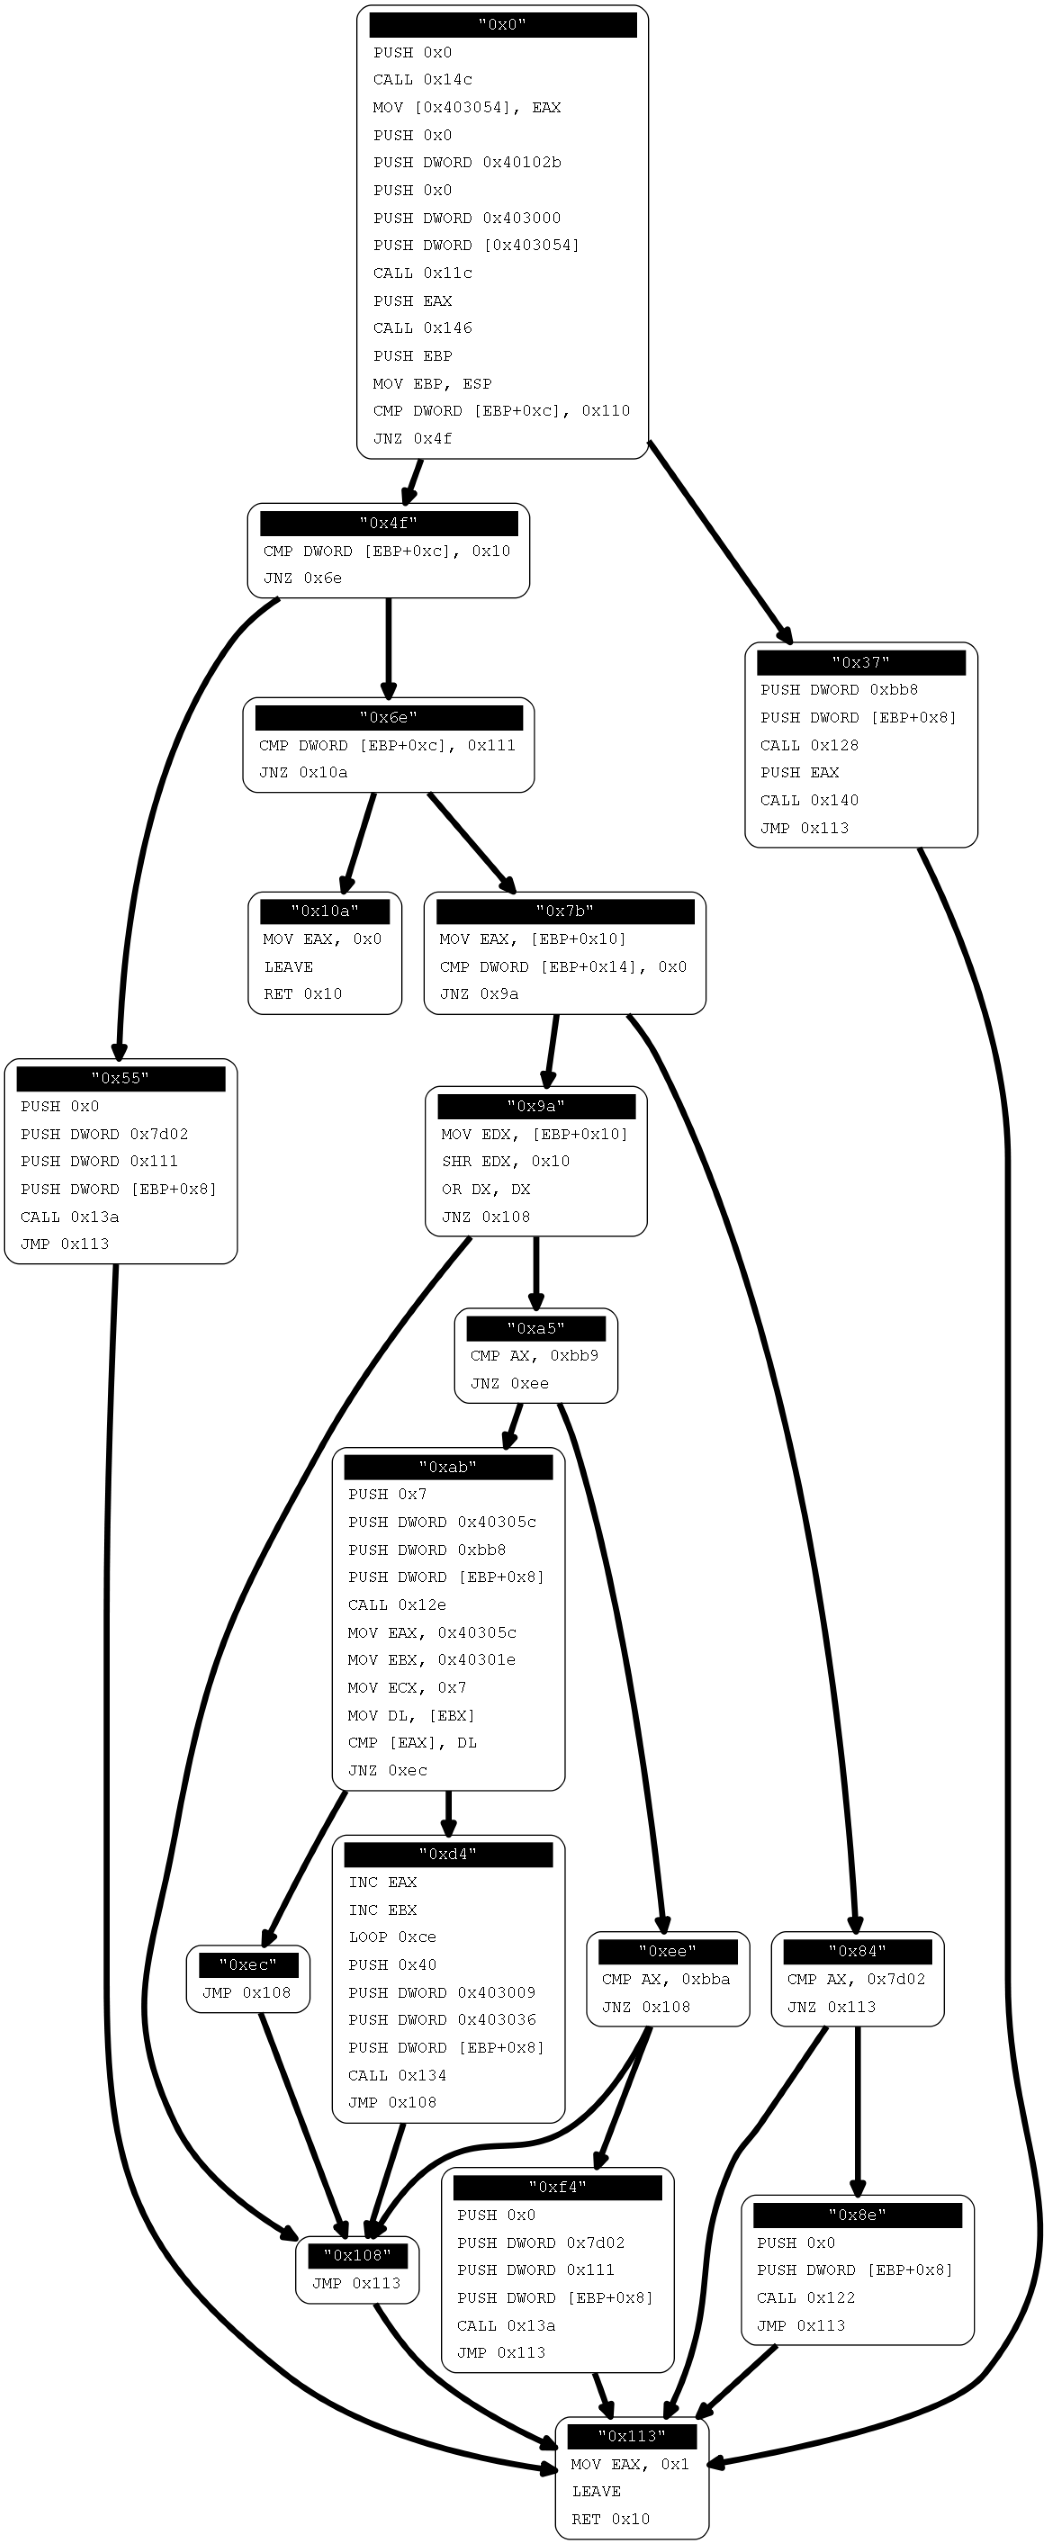
\includegraphics[width=\textwidth, height=\textheight]{slike/AD_CM1_graph}
\caption{Graf instrukcija za odsječak koda iz dodatka \ref{sct:appPE}}
\label{fig:appGraphInstr} 
\end{figure}
\clearpage

\begin{sazetak}
Korupcija memorije jedan je od najstarijih oblika ranjivosti koji
je danas još uvijek prisutan. Iako postoje mnogi mehanizmi
zaštite, problem korupcije memorije je i dalje dosta aktualan jer
se pojavom novih sigurnosnih mehanizama pojavljuju i nove metode
napada. Randomizacijski postupci značajno su pripomogli u borbi
protiv napada usmjerenih na memoriju, ali prostora za poboljšanje
još uvijek ima. Upravo je u ovome radu započet razvoj na jednom
novom randomizacijskom mehanizmu zaštite čiji cilj je provesti
permutaciju nad memorijskim blokovima unutar sekcije s izvršnim
kodom. Time bi se razina sigurnosti protiv navedenih oblika
napada podigla na jednu novu razinu.

\kljucnerijeci{PE format, računalna sigurnost, operacijski sustavi, ASLR, DEP, ASLP, randomizacija, korupcija memorije, permutacija, graf programskog toka, Microsoft Windows}
\end{sazetak}

% TODO: Navedite naslov na engleskom jeziku.
\engtitle{Development of an assembly source code permutation engine to improve application security against malicious applications}
\begin{abstract}
Memory corruption is one of the oldest security vulnerabilities
out there that is still very common today. Randomization based
security mechanisms had a major impact on dealing with memory
corruption vulnerabilities but the threat still remains. In this
paper we started work on a new randomization security mechanism
whose goal is to rearrange memory blocks in the code section of a
PE file. In that way, we could achieve higher security levels in
the system.

\keywords{PE file format, computer security, operating systems, ASLR, DEP, ASLP, randomization, memory corruption, permutation, control flow graph, Microsoft Windows}
\end{abstract}

\end{document}
